% Chapter Template

\chapter{Dependency-based Hybrid Trees for Semantic Parsing} % Main chapter title

\label{Chapter6} % Change X to a consecutive number; for referencing this chapter elsewhere, use \ref{ChapterX}

%----------------------------------------------------------------------------------------
%	SECTION 1
%----------------------------------------------------------------------------------------

\section{Introduction}
\label{sec:intro}

Semantic parsing is a fundamental task within the field of natural language processing (NLP).
Consider a natural language (NL) sentence and its corresponding meaning representation (MR) as illustrated in Figure \ref{fig:dhtexample}.
%Semantic parsing is the task of transforming the former to the latter  automatically.
Semantic parsing aims to transform the natural language sentences into machine interpretable meaning representations automatically. 
The task has been popular for decades and keeps receiving significant attention from the NLP community. 
Various systems~\cite{zelle1996learning,kate2005learning,zettlemoyer2005learning,liang11learning} were proposed over the years to deal with different types of semantic representations.
Such models include structure-based models~\cite{wong2006learning,lu2008generative,kwiatkowski2010inducing,jones2012semantic}  and neural network based models~\cite{dong2016language,cheng2017learning}. 


\begin{figure}[h!]
	\centering
	\scalebox{1}{
		\begin{tikzpicture}[node distance=2.0mm and 2.5mm, >=Stealth, 
		semantic/.style={draw=none, minimum height=5mm, rectangle},
		word/.style={draw=none, minimum height=5mm, rectangle},
		olabel/.style={draw=none, circle, minimum height=9mm, minimum width=9mm,line width=1pt, inner sep=2pt, fill=lowblue, text=fontgray, label={center:\textsc{o}}},
		bperlabel/.style={draw=none, circle, minimum height=9mm, minimum width=9mm,line width=1pt, inner sep=2pt, fill=lowblue, text=black, label={center:\textsc{per}}},
		borglabel/.style={draw=none, circle, minimum height=9mm, minimum width=9mm,line width=1pt, inner sep=2pt, fill=lowblue, text=black, label={center:\textsc{org}}},
		bgpelabel/.style={draw=none, circle, minimum height=9mm, minimum width=9mm,line width=1pt, inner sep=2pt, fill=lowblue, text=black, label={center:\textsc{Misc}}},
		nnlabel/.style={draw=none, circle, minimum height=9mm, minimum width=9mm,line width=1pt, inner sep=2pt, fill=mypumpkin, text=black, label={center:\textsc{Gpe}}},
		invis/.style={draw=none, circle, minimum height=9mm, minimum width=9mm,line width=1pt, inner sep=2pt, fill=none, text=fontgray},
		chainLine/.style={line width=1pt,-, color=fontgray}	%		,background rectangle/.style={fill=olive!45}, show background rectangle
		]
		
		\node[semantic](s1) [] {NL: What rivers do not run through Tennessee ?};
		\node[semantic](mr1) [below= of s1, yshift=2mm] {MR: $answer(exclude(river(all), traverse(stateid('tn'))))$}; 
		\node[draw=black, minimum height=47mm, minimum width=100mm, rectangle, line width=0.8pt, rounded corners] (box) [yshift=-27.5mm] {};
		
		\node[word](m1) [below left = of s1, yshift = -4mm, xshift=15mm] {$m_1$};
		\node[word](m2) [below=of m1, yshift=-2.5mm] {$m_2$};
		\node[word](m3) [below left=of m2, yshift=-1mm,xshift=-2.5mm] {$m_3$};
		\node[word](m4) [below right=of m2, yshift=-1mm, xshift=2.5mm] {$m_4$};
		\node[word](m5) [below =of m4, yshift=-2.5mm] {$m_5$};
		\node[word](m6) [below =of m5, yshift=-2.5mm] {$m_6$};
		
		\node[word](m1r)[right= of m1, xshift=12mm, yshift=-7mm] {$m_1$: Q{\small{UERY}} : $answer$ (R{\small{IVER}})};
		\node[word](m2r)[below= of m1r, yshift=4mm, xshift=5.5mm] {$m_2$: R{\small{IVER}} : $exclude$ (R{\small{IVER}}, R{\small{IVER}})};
		\node[word](m3r)[below= of m2r, yshift=4mm, xshift=-11.2mm] {$m_3$: R{\small{IVER}} : $river$ (all)};
		\node[word](m4r)[below= of m3r, yshift=4mm, xshift=5.9mm] {$m_4$: R{\small{IVER}} : $traverse$ (S{\small{TATE}})};
		\node[word](m5r)[below= of m4r, yshift=4mm, xshift=3.3mm] {$m_5$: S{\small{TATE}} : $stateid$ (S{\small{TATE}}N{\small{AME}})};
		\node[word](m6r)[below= of m5r, yshift=4mm, xshift=-1.8mm] {$m_6$: S{\small{TATE}}N{\small{AME}} : ($'tennessee'$)};
		
		\draw [line width=0.8pt,->, color=fontgray]  (m1) to [] node[]{} (m2);
		\draw [line width=0.8pt,->, color=fontgray]  (m2) to [] node[]{} (m3);
		\draw [line width=0.8pt,->, color=fontgray]  (m2) to [] node[]{} (m4);
		\draw [line width=0.8pt,->, color=fontgray]  (m4) to [] node[]{} (m5);
		\draw [line width=0.8pt,->, color=fontgray]  (m5) to [] node[]{} (m6);
		
		%		\Tree [.\node(root){$m_1$: Q{\small{UERY}} : $answer$ (R{\small{IVER}})}; [.{$m_2$: R{\small{IVER}}: $exclude$ (R{\small{IVER}}, R{\small{IVER}})} {$m_3 \equiv$ R{\small{IVER}} : $state$ (all)} [.{$m_4 \equiv$ R{\small{IVER}} : $traverse$ (S{\small{TATE}})} [.{$m_5 \equiv $S{\small{TATE}} : $stateid$ (S{\small{TATE}}N{\small{AME}})} {$m_6 \equiv$  S{\small{TATE}}N{\small{AME}} : ($'tennessee'$)} ]] ]]
		
		\node[word](w0) [below = of s1, xshift = -48mm, yshift=-62.5mm] {root};
		\node[word](w1) [right = of w0] {{\em What}};
		\node[invis](rootop) [above = of w0, yshift=8mm] {};
		\node[word](w2) [right = of w1] {{\em rivers}};
		\node[word](w3) [right = of w2] {{\em do}};
		\node[word](w4) [right = of w3] {{\em not}};
		\node[word](w5) [right = of w4] {{\em run}};
		\node[word](w6) [right = of w5] {{\em through}};
		\node[word](w7) [right = of w6] {{\em Tennessee}};
		\node[word](w8) [right = of w7] {{\em ?}};
		
		\draw [line width=0.8pt,->, color=fontgray]  (w0) to [out=60,in=120, looseness=1] node[above, yshift=0mm, color=black]{$m_1$} (w1);
		\draw [line width=0.8pt,->, color=fontgray]  (w1) to [out=60,in=120, looseness=1] node[above, color=black]{$m_2$} (w4);
		\draw [line width=0.8pt,->, color=fontgray]  (w4) to [out=130,in=60, looseness=1] node[above, yshift=-1mm, color=black]{$m_3$} (w2);
		\draw [line width=0.8pt,->, color=fontgray]  (w4) to [out=60,in=120, looseness=1] node[above, yshift=-1mm, color=black]{$m_4$} (w6);
		\draw [line width=0.8pt,->, color=fontgray]  (w6) to [out=60,in=120, looseness=1] node[above, yshift=-1mm, color=black]{$m_5$} (w7);
		\draw [line width=0.8pt,->, color=fontgray]  (w7) to [out=90,in=30, looseness=4.8] node[above, yshift=-1mm, color=black]{$m_6$} (w7);
		%		\draw[line width=0.8pt,->, color=fontgray] (w6.0) arc (90:180+264:4mm);
		%		\node[semantic](s2) [below= of w4] {{\em What} ({\em not} ({\em rivers}, ({\em through} ({\em Tennessee}))))};
		\end{tikzpicture} 
	}
	%	\vspace{-2mm}
	\caption{Top: natural language (NL) sentence; middle: meaning representation (MR); bottom:  dependency-based hybrid tree representation.}
	%	\vspace{1mm}
	%	\vspace{-5mm}
	\label{fig:dhtexample}
\end{figure}

Following various previous research efforts \cite{wong2006learning,lu2008generative,jones2012semantic},  in this work, we adopt a popular class of semantic formalism -- logical forms that can be equivalently represented as tree structures.
The  tree representation of an example MR is shown in the middle of Figure \ref{fig:example}.
One challenge associated with building a semantic parser is that the exact correspondence between the words and atomic semantic units are not explicitly given during the training phase.
The key to the building of a successful semantic parsing model lies in the identification of a good {\em joint} latent representation of both the sentence and its corresponding semantics.
Example joint representations proposed in the literature include a chart used in phrase-based translation \cite{wong2006learning}, a constituency tree-like representation known as {\em hybrid tree} \cite{lu2008generative}, and a CCG-based derivation tree \cite{kwiatkowski2010inducing}.

Previous research efforts have shown the effectiveness of using dependency structures to extract semantic representations~\cite{debusmann2004relational,cimiano2009flexible,bedaride2011deep,stanovsky2016getting}. 
Recently, \citet{reddy2016transforming,reddy2017universal} proposed a model to construct logical representations from sentences that are parsed into dependency structures.
Their work demonstrates the connection between the dependency structures of a sentence and its underlying semantics.
Although their setup and objectives are different from ours where externally trained dependency parsers are assumed available and their system was trained to use the semantics for a specific down-stream task, the success of their work motivates us to propose a novel joint  representation that can explicitly capture dependency structures among words for the semantic parsing task.

%Various semantic formalisms have been used in semantic parsing: tree-structured semantic representations~\cite{kate2006using,wong2006learning}, the lambda-calculus logical form~\cite{zettlemoyer2005learning,wong2007learning} and dependency-based semantic representations (DCS)~\cite{liang2013learning}. 
%Consider the meaning representation in the form of tree structure shown in Figure \ref{fig:example}.
%In this work, we adopt the variable-free semantic representations where the underlying meaning representations (MR) can be expressed in the form of tree structures. 
%An example tree-structured meaning representation taken from the GeoQuery dataset is shown at the top of Figure \ref{fig:example}. 
%Each tree node in the semantic tree represents an atomic semantic unit $m_i$. 
%As shown in the middle of Figure \ref{fig:example}, the trees corresponds to the natural language (NL) sentences can be further represented as a string-form meaning representation (MR) via function composition. 
%We present more details of tree-structured semantic representation in Section \ref{sec:semantics}. 



%Figure \ref{fig:example} shows an example of such a tree-structured 
%Such semantics can be represented by tree structure as shown in Figure \ref{fig:example}. 
%Each node in the tree is an atomic semantic unit referred as $m$ for short. 
%More details of the tree-structured semantic representations are given in Section \ref{sec:semantics}. 


%Learning such tree-structured semantic representations is typically more challenging as the complete semantic trees are not explicitly associated (or aligned) to the natural language sentences. 
%In order to capture the interactions between the semantics and natural language sentences, we observe that the semantic units are actually related to some of the natural language words and can represent the directed relationship between the words. 
%As shown at the bottom of Figure \ref{fig:example}, we can jointly represent the semantic representation and the natural language sentence into a dependency tree where the semantic units are interpreted as the dependency (or relationship) between two words\footnote{We introduce a special token ``{\em root}'' to represent the root of a dependency tree.}. 
%We call the resulting joint representation {\em dependency-based hybrid tree} (\textsc{DepHT}).
%For example, $m_2$ (i.e., R{\small{IVER}}: $exclude$ (R{\small{IVER}}, R{\small{IVER}})) is the relation of the dependency from the parent ``{\em What}'' to the child ``{\em not}''. 
%On the other hand, the words (i.e., ``{\em What rivers do not}'') that covered by this dependency arc also explicitly express the semantic unit $m_2$. 
%Such {\em parent-child dependency} and {\em span-level semantic information} are highly meaningful to connect the underlying semantic representation and the natural language sentences. 
%The {\em span-level semantic information} was shown to be effective in the semantic parsing task~\cite{kwiatkowski2010inducing,liang2013learning,lu2014semantic,susanto2017semantic}. 

%Additionally, with the representation of {\em dependency-based hybrid tree}, we can perceive how the underlying semantics express and change upon the natural language words by following the dependency tree. 
%Specifically, we can further extract a variable-free logical representation using natural language words from the {\em dependency-based hybrid tree} in Figure \ref{fig:example}:
%\begin{figure}[h!]
%	\centering
%	\scalebox{0.8}{
%		\begin{tikzpicture}[node distance=2.0mm and 2.5mm, >=Stealth, 
%		semantic/.style={draw=none, minimum height=5mm, rectangle},
%		]
%		\node[semantic](s1) [] {{\em What} ({\em not} ({\em rivers}, ({\em through} ({\em Tennessee}))))};
%		\node[semantic](mr1) [below= of s1, yshift=3mm] {MR: $answer(exclude(river(all), traverse(stateid('tn'))))$}; 
%		\end{tikzpicture} 
%	}
%	\vspace*{-7mm}
%\end{figure}

%\noindent We can see that the extracted variable-free logical expression from the words is similar to the meaning representation in a sense that the functional words have similar meanings, which makes our {\em dependency-based hybrid tree} have a decent interpretability on the meaning representation. 
%%the advantage of interpreting the meaning representation.   
%
%As such useful dependencies are not given in semantic parsing tasks, we model them as latent variables and the semantics are the latent dependencies between the natural language words. 
%Note that our task is different from semantic dependency parsing~\cite{oepen2015semeval} SemEval shared task, which is the task of recovering predicate-argument relationships and related to semantic role labeling. 


%We propose a novel {\em dependency-based hybrid tree} representation, a new joint latent structured representation of both semantics and natural language sentences. 
%Most of previous work~\cite{liang11learning,dong2016language,cheng2017learning,susanto2017neural} model the semantic representations without explicitly capturing the interactions between the semantics and natural language words, which potentially makes the system/model less interpretable. 
%\citet{lu2014semantic} proposed a \textit{relaxed hybrid tree} model which capture span-level interactions between the semantic units and natural language words as well as the long-distance dependencies. 
%\citet{reddy2016transforming} deterministically transforms the syntactic dependencies into logical forms and the results depend on the quality from dependency parsing. 
%Inspired by both literatures, we propose a novel latent semantic representations involved the natural language words as shown in the bottom of Figure \ref{fig:example}. 
%The semantics are modeled as latent dependency trees over natural language words. 
%We believe such representations capture span-level interactions as in \cite{lu2014semantic} and we do not require external syntactic dependency parsers to build semantic representations as in \cite{reddy2016transforming}. 
%For example, ``\textit{What rivers do not}'' is covered by the arc from ``\textit{What}'' to ``\textit{not}'' and corresponding semantic unit is  $m_2$ (i.e., R{\small{IVER}}: $exclude$ (R{\small{IVER}}, R{\small{IVER}})). 
%Such information is similarly captured in hybrid tree model and the semantic information can be captured by dependencies between specific words. 
%Furthermore, it is clear to interpret the semantics following the dependency tree along the natural language words and semantic units. 
In this work, we propose a new joint representation for both semantics and words, presenting a new model for semantic parsing. 
Our main contributions can be summarized as follows: 
\begin{itemize}

\item We present a novel {\em dependency-based hybrid tree} representation that captures both words and semantics in a joint manner.
Such a dependency tree reveals semantic dependencies between words which are easily interpretable. 

%	\item We build a semantic parser with such a representation, presenting 
\item We show that exact dynamic programming algorithms for inference can be designed on top of our new representation.  We further show that the model can be integrated with neural networks for improved effectiveness.
%	propose a neural graphical model to learn the latent {\em dependency-based hybrid tree} structure. 
%		Our efficient dynamic-programming algorithm allows the model to perform tractable inference over the graphical model and the neural networks. 
\item Extensive experiments conducted on the standard multilingual GeoQuery dataset 
%	with eight languages
show that our model outperforms the state-of-the-art models on 7 out of 8 languages. Further analysis confirms the effectiveness of our  dependency-based representation.
\end{itemize}

To the best of our knowledge, this is the first work that models the semantics as latent dependencies between   words for semantic parsing. 

{\color{red}
	
}



\section{Related Work}
The literature on semantic parsing has focused on various types of semantic formalisms. 
The $\lambda$-calculus expressions~\cite{zettlemoyer2005learning} have been popular and widely used in semantic parsing tasks over recent years~\cite{dong2016language,gardner2017open,reddy2016transforming,reddy2017universal,susanto2017neural,cheng2017learning}. 
Dependency-based compositional semantics (DCS)\footnote{Unlike ours, their work captures dependencies between  semantic units but not natural language words.} was introduced by \citet{liang11learning}, whose extension, $\lambda$-DCS, was later proposed by \citet{liang2013lambda}. 
Various models~\cite{berant2013semantic,wang2015building,jia-liang:2016:P16-1}  on semantic parsing with the $\lambda$-DCS formalism were proposed. 
In this work, we focus on the tree-structured semantic formalism which has been examined by various research efforts~\cite{wong2006learning,kate2006using,lu2008generative,kwiatkowski2010inducing,jones2012semantic,lu2014semantic,yan2018learn}.

\citet{wong2006learning} proposed the \textsc{Wasp} semantic parser 
that regards the task as a phrase-based machine translation problem.
%using statistical phrase-based machine translation approach by regarding the mapping natural language words to semantic representations as an alignment problem. 
\citet{lu2008generative} proposed a generative process to generate natural language words and semantic units in a joint model. 
The resulting representation is called \textit{hybrid tree} where both natural language words and semantics are encoded into a joint representation. 
The \textsc{UBL}-s~\cite{kwiatkowski2010inducing} parser applied the CCG grammar~\cite{steedman1996surface} to model the joint representation of both semantic units and contiguous word sequences which do not overlap with one another. 
\citet{jones2012semantic} applied a generative process with Bayesian tree transducer and their model also simultaneously generates the meaning representations and natural language words. 
\citet{lu2014semantic,lu2015constrained} proposed a discriminative version of the hybrid tree model of \cite{lu2008generative} where richer features can be captured. 
\citet{dong2016language} proposed a sequence-to-tree model using recurrent neural networks where the decoder can branch out to produce tree structures. 
\citet{susanto2017semantic} augmented the discriminative {hybrid tree} model with multilayer perceptron and achieved state-of-the-art performance. 




There exists another line of work that applies given syntactic dependency information to semantic parsing. 
\citet{titov2011bayesian} decomposed a syntactic dependency tree into fragments and modeled the semantics as relations between the fragments. 
\citet{poon2013grounded} learned to derive semantic structures based on syntactic dependency trees predicted by the Stanford dependency parser.
%modeled the semantic units on syntactic dependency-tree nodes and edges.
\citet{reddy2016transforming,reddy2017universal} proposed a linguistically motivated procedure to transform syntactic dependencies into logical forms. 
Their semantic parsing performance relies on the quality of the syntactic dependencies.
Unlike such efforts, we do not require external syntactic dependencies, but model the semantic units as latent dependencies between natural language words. 

\section{Approach}

%OK

%We briefly describe the variable-free semantics and introduce our {\em dependency-based hybrid tree} model in this section. 
%We further present a dynamic-programing algorithm to allow tractable inference during training and decoding. 

\subsection{Variable-free Semantics}
\label{sec:semantics}
The variable-free semantic representations in the form of FunQL~\cite{kate2005learning} used by the de-facto GeoQuery dataset~\cite{zelle1996learning} encode semantic compositionality of the logical forms~\cite{cheng2017learning}. 
In the tree-structured semantic representations as illustrated in Figure \ref{fig:example}, each tree node is a semantic unit of the following form:
\begin{equation*}
m_i \equiv \tau_\alpha : p_\alpha(\tau_\beta ^ *)
\end{equation*}
%\begin{center}
%	\begin{tabular}{c}
%		$
%		m_i \equiv \tau_\alpha : p_\alpha(\tau_\beta ^ *)
%		$
%	\end{tabular}
%\end{center}
where $m_i$ denotes the complete semantic unit, which consists of semantic type $\tau_\alpha$, function symbol $p_\alpha$ and an argument list of semantic types $\tau_\beta^*$ (here $*$ denotes that there can be 0, 1, or 2 semantic types in the  argument list. This number is known as the {\em arity} of $m_i$). 
Each semantic unit can be regarded as a function that takes in other (partial) semantic representations of certain types as arguments and returns a semantic representation of a specific type.
For example in Figure \ref{fig:example}, the root unit is represented by $m_1$, the type of this unit is \textsc{Query}, the function name is $answer$ and it has a single argument  \textsc{River} which is a semantic type. 
With  recursive function composition, we can obtain a complete MR as shown in Figure \ref{fig:example}.
%In our dependency-based representation, each semantic unit serves as the dependency label between the natural language words as shown at the bottom of Figure \ref{fig:example}. 

\subsection{Dependency-based Hybrid Trees}
To jointly encode the tree-structured semantics $\boldsymbol{m}$ and a natural language sentence $\boldsymbol{n}$, we introduce our novel {\em dependency-based hybrid tree}. 
Figure \ref{fig:dhtexample} (right) shows the two equivalent ways of visualizing the {dependency-based hybrid tree} based on the example given in Figure \ref{fig:example}. 
In this example, the bold symbol $\boldsymbol{m}$ is the tree-structured semantics $m_1 (m_2 (m_3, m_4(m_5(m_6))))$ and $\boldsymbol{n}$ is the sentence $\{w_1, w_2, \cdots,w_8\}$\footnote{We also introduce a special token ``{\em root}'' as $w_0$.}. 
Our {dependency-based hybrid tree} $\boldsymbol{t}$ consists of a set of dependencies  between the natural language words, each of which is labeled with a semantic unit. 
Formally, a dependency arc is represented as $(w_p, w_c, m_i)$, where $w_p$ is the {\em parent} of this dependency, $w_c$ is the {\em child}, and $m_i$ is the semantic unit that serves as the {\em label} for the dependency arc. 
A valid dependency-based hybrid tree (with respect to a given semantic representation) allows one to recover the correct semantics from it.
Thus, one constraint is that for any two adjacent dependencies $(w_p, w_c, m_i)$ and $(w_p^\prime, w_c^\prime, m_j)$, where $w_c \equiv w_p^\prime$, $m_i$ must be the parent of $m_j$ in the tree-structured representation $\boldsymbol{m}$.  
For example, in Figure \ref{fig:dhtexample}, the dependencies ({\em not}, {\em through}, $m_4$) and ({\em through}, {\em Tennessee}, $m_5$) satisfy the above condition. 
However, we cannot replace ({\em through}, {\em Tennessee}, $m_5$) with, for example, ({\em through}, {\em Tennessee}, $m_6$), since $m_6$ is not the child of $m_4$. 
Furthermore, the number of children for a word in the dependency tree should be consistent with the arity of the corresponding semantic unit that points to it. 
For example, ``{\em not}'' has 2 children in our {dependency-based hybrid tree} representation because the semantic unit $m_2$ (i.e., R{\small{IVER}} : $exclude$ (R{\small{IVER}}, R{\small{IVER}})) has arity 2. 
Also, ``{\em rivers}'' is the leaf as $m_3$, which points to it, has arity 0.
We will discuss in Section \ref{sec:patterns} on how to derive the set of allowable dependency-based hybrid trees for a given $(\boldsymbol{m},\boldsymbol{n})$ pair.
% and has no child.
%no semantic unit argument.





To understand the potential advantages of our new joint representation, we compare it with the {\em relaxed hybrid tree} representation~\cite{lu2014semantic}, which is illustrated on the left of Figure \ref{fig:dhtexample}.
We highlight some similarities and differences between the two representations from the {\em span level} and {\em word level} perspectives.

\begin{figure*}[h!]
	\centering
	\scalebox{0.75}{
		\begin{tikzpicture}[node distance=2.0mm and 2.5mm, >=Stealth, 
		semantic/.style={draw=none, minimum height=5mm, rectangle},
		word/.style={draw=none, minimum height=5mm, rectangle},
		olabel/.style={draw=none, circle, minimum height=9mm, minimum width=9mm,line width=1pt, inner sep=2pt, fill=lowblue, text=fontgray, label={center:\textsc{o}}},
		bperlabel/.style={draw=none, circle, minimum height=9mm, minimum width=9mm,line width=1pt, inner sep=2pt, fill=lowblue, text=black, label={center:\textsc{per}}},
		borglabel/.style={draw=none, circle, minimum height=9mm, minimum width=9mm,line width=1pt, inner sep=2pt, fill=lowblue, text=black, label={center:\textsc{org}}},
		bgpelabel/.style={draw=none, circle, minimum height=9mm, minimum width=9mm,line width=1pt, inner sep=2pt, fill=lowblue, text=black, label={center:\textsc{Misc}}},
		nnlabel/.style={draw=none, circle, minimum height=9mm, minimum width=9mm,line width=1pt, inner sep=2pt, fill=mypumpkin, text=black, label={center:\textsc{Gpe}}},
		invis/.style={draw=none, circle, minimum height=9mm, minimum width=9mm,line width=1pt, inner sep=2pt, fill=none, text=fontgray},
		chainLine/.style={line width=0.8pt,->, color=fontgray}	%		,background rectangle/.style={fill=olive!45}, show background rectangle
		]
		\node[semantic](sent) [] {Sentence: {\em What rivers do not run through Tennessee ?}}; 
		
		\node[word](htname) [below left = of sent, xshift=0mm] {{\em Relaxed Hybrid Tree}};
		
		\node[word](hm1) [below = of htname, xshift=0mm] {$m_1$};
		\node[word](hw1) [below left = of hm1, xshift=-20mm, yshift=-3mm] {{\em What}};
		\node[word](hw8) [below right = of hm1, xshift=35mm, yshift=-3mm] {{\em ?}};
		\node[word](hm2) [below = of hm1, xshift=0mm, yshift=-3mm] {$m_2$};
		
		\node[word](hm3) [below left= of hm2, xshift=-8mm, yshift=-3mm] {$m_3$};
		\node[word](hm4) [below right= of hm2, xshift=14mm, yshift=-3mm] {$m_4$};
		\node[word](hw34) [below= of hm2, xshift=0mm, yshift=-3mm] {{\em do not}};
		
		\node[word](hw2) [below= of hm3, xshift=0mm, yshift=-3mm] {{\em rivers}};
		
		\node[word](hm5) [below right= of hm4, xshift=5mm, yshift=-3mm] {$m_5$};
		\node[word](hw56) [below left= of hm4, xshift=2mm, yshift=-3mm] {{\em run through}};
		\node[word](hm6) [below= of hm5, xshift=0mm, yshift=-3mm] {$m_6$};
		\node[word](hw7) [below= of hm6, xshift=0mm, yshift=-3mm] {{\em Tennessee}};
		
		\draw [chainLine] (hm1) to [] node[] {} (hw1);
		\draw [chainLine] (hm1) to [] node[] {} (hm2);
		\draw [chainLine] (hm1) to [] node[] {} (hw8);
		
		\draw [chainLine] (hm2) to [] node[] {} (hm3);
		\draw [chainLine] (hm2) to [] node[] {} (hw34);
		\draw [chainLine] (hm2) to [] node[] {} (hm4);
		
		\draw [chainLine] (hm3) to [] node[] {} (hw2);
		\draw [chainLine] (hm4) to [] node[] {} (hw56);
		\draw [chainLine] (hm4) to [] node[] {} (hm5);
		
		\draw [chainLine] (hm5) to [] node[] {} (hm6);
		\draw [chainLine] (hm6) to [] node[] {} (hw7);
		
		
		\node[word](dhtname) [below right = of sent, xshift=-48mm] {{\em Dependency-based Hybrid Tree}};
		\node[word](root) [below = of dhtname, xshift=-5mm] {\textit{root}};
		\node[word](what) [below left = of root, yshift=-3mm, xshift=-3mm] {\textit{What}};
		%		\node[invis](rootop) [above = of w0, yshift=8mm] {};
		\node[word](not) [below right = of what, xshift=15mm, yshift=3mm] {\textit{not}};
		\node[word](rivers) [below left = of not, yshift=-4mm] {\textit{rivers}};
		\node[word](through) [below right = of not, yshift=-4mm] {\textit{through}};
		\node[word](tennessee) [below right = of through, yshift=-4mm, xshift=-2mm] {\textit{Tennessee}};
		
		\node[word](m1)[right= of root, xshift=24mm, yshift=2mm] {$m_1$: Q{\small{UERY}} : $answer$ (R{\small{IVER}})};
		\node[word](m2)[below= of m1, yshift=4mm, xshift=5.5mm] {$m_2$: R{\small{IVER}} : $exclude$ (R{\small{IVER}}, R{\small{IVER}})};
		\node[word](m3)[below= of m2, yshift=4mm, xshift=-11.2mm] {$m_3$: R{\small{IVER}} : $state$ (all)};
		\node[word](m4)[below= of m3, yshift=4mm, xshift=5.9mm] {$m_4$: R{\small{IVER}} : $traverse$ (S{\small{TATE}})};
		\node[word](m5)[below= of m4, yshift=4mm, xshift=3.3mm] {$m_5$: S{\small{TATE}} : $stateid$ (S{\small{TATE}}N{\small{AME}})};
		\node[word](m6)[below= of m5, yshift=4mm, xshift=-1.8mm] {$m_6$: S{\small{TATE}}N{\small{AME}} : ($'tennessee'$)};
		
		%		\Tree [.\node(root){$m_1 \equiv $ Q{\small{UERY}} : $answer$ (R{\small{IVER}})}; [.{$m_2 \equiv $ R{\small{IVER}}: $exclude$ (R{\small{IVER}}, R{\small{IVER}})} {$m_3 \equiv$ R{\small{IVER}} : $state$ (all)} [.{$m_4 \equiv$ R{\small{IVER}} : $traverse$ (S{\small{TATE}})} [.{$m_5 \equiv $S{\small{TATE}} : $stateid$ (S{\small{TATE}}N{\small{AME}})} {$m_6 \equiv$  S{\small{TATE}}N{\small{AME}} : ($'texas'$)} ]] ]]
		
		\draw [chainLine] (root) to [] node[above, color=black,sloped] {\small  $m_1$} (what);
		\draw [chainLine] (what) to [] node[above, color=black,sloped] {\small  $m_2$} (not);
		\draw [chainLine] (not) to [] node[above, color=black,sloped] {\small  $m_3$} (rivers);
		\draw [chainLine] (not) to [] node[above, color=black,sloped] {\small  $m_4$} (through);
		\draw [chainLine] (through) to [] node[above, color=black,sloped] {\small  $m_5$} (tennessee);
		\draw [line width=0.8pt,->, color=fontgray]  (tennessee) to [out=90,in=-30, looseness=5.2] node[above, yshift=-1mm, color=black, sloped]{$m_6$} (tennessee);
		
		\node[word](wroot) [below = of sent, xshift = 5mm, yshift=-64mm] {{\em root}};
		\node[word](w0) [right = of wroot] {{\em What}};
		%		\node[invis](rootop) [above = of w0, yshift=8mm] {};
		\node[word](w1) [right = of w0] {{\em rivers}};
		\node[word](w2) [right = of w1] {{\em do}};
		\node[word](w3) [right = of w2] {{\em not}};
		\node[word](w4) [right = of w3] {{\em run}};
		\node[word](w5) [right = of w4] {{\em through}};
		\node[word](w6) [right = of w5] {{\em Tennessee}};
		\node[word](w7) [right = of w6] {{\em ?}};
		
		\draw [line width=0.8pt,->, color=fontgray]  (wroot) to [out=60,in=120, looseness=1] node[above, yshift=2mm, color=black]{$m_1$} (w0);
		\draw [line width=0.8pt,->, color=fontgray]  (w0) to [out=60,in=120, looseness=1] node[above, color=black]{$m_2$} (w3);
		\draw [line width=0.8pt,->, color=fontgray]  (w3) to [out=130,in=60, looseness=1] node[above, yshift=-1mm, color=black]{$m_3$} (w1);
		\draw [line width=0.8pt,->, color=fontgray]  (w3) to [out=60,in=120, looseness=1] node[above, yshift=-1mm, color=black]{$m_4$} (w5);
		\draw [line width=0.8pt,->, color=fontgray]  (w5) to [out=60,in=120, looseness=1] node[above, yshift=-1mm, color=black]{$m_5$} (w6);
		\draw [line width=0.8pt,->, color=fontgray]  (w6) to [out=90,in=30, looseness=4.8] node[above, yshift=-1mm, color=black]{$m_6$} (w6);
		\end{tikzpicture} 
	}
	%	\vspace*{-3mm}
	\caption{The \textit{relaxed hybrid tree} (left)~\cite{lu2014semantic} and our {\em dependency-based hybrid tree} (right) as well as the flat representation (bottom right)  of the example in Figure \ref{fig:example}.}
	%	\vspace*{-3mm}
	\label{fig:dhtexample}
\end{figure*}


%We highlight several properties of our representation has but is not present in their representation.
% relaxed hybrid tree} representation does not hold: span-level semantic information and parent-child dependency. 
%In a {relaxed hybrid tree}, each tree node can be represented as a pair consisting of a semantic unit and a span of words  it covers, where some words in the span are directly related to the semantic unit and some are not\footnote{We refer readers to \cite{lu2014semantic} for more details.}. 
In a relaxed hybrid tree representation, words and semantic units jointly form a constituency tree-like structure, where the former are  leaves and the latter are internal nodes of such a joint representation.
Such a representation is able to capture alignment between the natural language words and semantics at the span level.\footnote{We refer readers to \cite{lu2014semantic} for more details.}
%For example in Figure \ref{fig:dhtexample}, a {\em relaxed hybrid tree} representation is shown on the left. 
For example, $m_2$ covers the span from ``{\em rivers}'' to ``{\em Tennessee}'', which allows the interactions between the semantic unit and the span to be captured.
%For example, the words ``{\em do not}'' are immediately associated with $m_2$ which captures the meaning of this sub-span. 
%Also, ``{\em run through}'' is immediately associated with $m_4$. 
Similarly, in our {dependency-based hybrid tree}, 
such span level word-semantics correspondence can also be captured. 
For example, the arc between ``{\em not}'' and ``{\em through}'' is labeled by the semantic unit $m_4$.
This also allows the interactions between $m_4$ and words within the span from ``{\em not}'' to ``{\em through}'' to be captured.
%``{\em not}'' is the child under the dependency arc labeled with semantic unit $m_2$ and ``{\em through}'' is the child under the dependency arc labeled with $m_4$. 




While both models are able to capture the span-level correspondence between words and semantics,
we can observe that in the relaxed hybrid tree, some words within the span are more directly related to the semantic unit (e.g., ``{\em do not}'' are more related to $m_2$) and some are not.
%we can, however, observe that the span covered by $m_2$ in {relaxed hybrid tree} contains many of the words in the sentence, which may not be semantically related to $m_2$ (i.e., R{\small{IVER}} : $exclude$ (R{\small{IVER}}, R{\small{IVER}})). 
Specifically, in their representation, the span level information assigned to the parent semantic unit always contains the span level information assigned to all its child semantic units.
This may not always be desirable and may lead to irrelevant features.
In fact, \citet{lu2014semantic} also empirically showed that the span-level features may not always be helpful in their representation.
In contrast, in our {dependency-based hybrid tree}, the span covered by $m_2$ is from ``{\em What}'' to ``{\em not}'', which only consists of the span level information associated with its first child semantic units.
Therefore, our representation is more flexible in capturing the correspondence between words and semantics at the span level, allowing the model to choose the relevant span for features.
%allows us to select the most relevant span for building features.

%which only covers information relevant to the first argument 
%, whose information is more precise to the semantic unit $m_2$. 

Furthermore, our representation can also capture precise interactions between words through  dependency arcs labeled with semantic units.
%also capture more specific semantics as dependencies between words. 
For example, the semantic unit $m_4$ on the dependency arc from  ``{\em not}'' to ``{\em through}'' in our representation can be used to capture their interactions. 
However, such information could not be straightforwardly captured in a relaxed hybrid tree, which is essentially a constituency tree-like representation.
% largely focuses on capturing dependencies between words (or phrases, which serve as terminal nodes) and semantic units (which are non-terminal nodes).
In the same example, consider the word ``{\em not}'' that bridges  two arcs labeled by $m_2$ and $m_4$. 
Lexical features defined over such arcs can be used to indirectly capture the interactions between  semantic units and guide the tree construction process.
% the interaction between {\em not} and $m_2$ is captured with a dependency arc. 
%Together with the $m_4$ arc, we will be able to indirectly capture the interaction between $m_2$ and $m_4$ through such lexical features. 
%This makes our joint representation similar to an implicit lexicalized dependency tree.
We believe such properties can be beneficial in practice, especially for certain languages. We will examine their significance   in our experiments later.
%We believe such word-word interactions could be useful, especially for certain languages, as we will discuss later in the experiments.
%indicates the antisense of $m_4$ (i.e. $traverse$) where as $m_4$ is not correlated to ``{\em not}'' in the {\em relaxed hybrid tree} representation. 

%The representation encodes the semantic units $m_i$ and natural language words into a single dependency tree. 
%The dependency tree is rooted at a special ``\textit{root}'' token, which is similar to dependency parsing~\cite{koo2010efficient}. 
%For example, an edge from ``\textit{root}'' to ``\textit{What}'' has a dependency relation $m_1$ -- indicating the semantic unit ``Q{\small{UERY}} : $answer$ (R{\small{IVER}})'' is related to the question word ``\textit{What}''. 
%Similarly, the dependency from ``\textit{What}'' to ``\textit{not}'' have relation ``R{\small{IVER}} : $exclude$ (R{\small{IVER}}, R{\small{IVER}})''. 
%We can also observe that the span covered by this dependency in the sentence is ``\textit{What rivers do not}'', which is also an interpretation from the the semantic unit $m_2$. 
%Following the path of dependency trees, we can understand how the semantic units interpret the natural language words.
%\textbf{Need some formulation} 
%
%Additionally, unlike traditional dependency trees where each word must and only have one parent, our representation is more flexible. 
%Due to the nature that the number of semantic units does not depend on the number of words, we allows some of the words have no parent and recurrence of dependencies on a word itself. 
%For example in Figure \ref{fig:dhtexample}, ``\textit{do}'', ``\textit{run}'' and ``\textit{?}'' have no parents in our dependency tree structure. 
%But we can still capture their semantic information by the dependency arcs cover them. 
%For the word ``\textit{Tennessee}'', which is related to both semantic units $m_5$ and $m_6$, it's reasonable to have such recurrence to capture these semantics. 
%We can set a maximum height to restrict the length of those recurrences\footnote{Similar strategy is used in the \textit{constrained hybrid tree} model~\cite{lu2015constrained}.}.
%To conclude, there are some other possible dependency-based tree representations, the one in Figure \ref{fig:dhtexample} is one of them. 
%Further, our model is globally optimized


\subsection{Expressiveness of Dependency-based Hybrid Trees}
The original hybrid tree representation~\cite{lu2014semantic} belongs to the class of constituency parse tree~\cite{chomsky2002syntactic}.
The context-free grammars (CFGs) are able to precisely describe our languages and help us understand the complexity of languages~\cite{johnson1998pcfg}.
While a constituency parse tree represents the nesting of multi-word constituents, a dependency parse tree~\cite{kubler2009dependency} represents the dependencies between individual words.
There has been much discussion on the dependency grammars and the phrase structure grammars~\cite{miller1999strong}. 
Though the constituency parse trees have been dominant for years, the syntactic annotation has shifted the focus to the dependency structures\footnote{Up to now, we have 157 treebanks for 90 languages in Universal Dependencies.}~\cite{eisenstein2018natural}.
The dependency trees are able to describe the direct grammatical relations which can be extracted from the constituents in the phrase structure parse tree~\cite{de2006generating}.
Thus, we believe that there should be a formal discussion for the expressiveness of the proposed dependency-based hybrid tree representations compared with the hybrid tree representations.
Because our dependency-based hybrid trees are not exactly same as traditional dependency trees where each word is attached to exactly one parent.
We will leave the formal discussion for future work.
%First, the outer words always get aligned  earlier than the inner words.
%Secondly, the outer words should align with the semantic units with a larger height than the inner words.
%We know that such a structure can precisely describe languages that have relatively standard word order such as English. 
%However, such a structure might not be expressive enough to describe other languages with flexible word order.
%For example, the adjective words appear before the noun in English but appear after the noun in Italian. 
%Using the hybrid tree representation is difficult to describe the languages with flexible word order~\cite{ahmad2019difficulties}.
%Because the outer words would possibly align to the semantic units with smaller height than the inner words.
%With the dependency-based representation, the semantic units can directly align to the inner words without any constraint but we just need to make sure tree structure is \textit{projective}, which is often true for many languages~\cite{jurafsky2000speech}. 
%Because the number of semantic units does not always match the number of words in a sentence. 
%We allow that some of the words are not attached to any parents and some of the words would have a self-loop. 
%These properties actually make the representation more flexible to adapt to different languages with flexible word order.
%Therefore, the dependency-based hybrid tree representations are more expressive than the hybrid tree representations in terms of the word order.

%\subsection{Expressiveness of Dependency-based Hybrid Trees}
%As we can see,  the original hybrid tree representation~\cite{lu2014semantic} is isomorphic to the constituency parse tree~\cite{chomsky2002syntactic}.
%First, the outer words always get aligned  earlier than the inner words.
%Secondly, the outer words should align with the semantic units with a larger height than the inner words.
%We know that such a structure can precisely describe languages that have relatively standard word order such as English. 
%However, such a structure might not be expressive enough to describe other languages with flexible word order.
%For example, the adjective words appear before the noun in English but appear after the noun in Italian. 
%Using the hybrid tree representation is difficult to describe the languages with flexible word order~\cite{ahmad2019difficulties}.
%Because the outer words would possibly align to the semantic units with smaller height than the inner words.
%With the dependency-based representation, the semantic units can directly align to the inner words without any constraint but we just need to make sure tree structure is \textit{projective}, which is often true for many languages~\cite{jurafsky2000speech}. 
%Because the number of semantic units does not always match the number of words in a sentence. 
%We allow that some of the words are not attached to any parents and some of the words would have a self-loop. 
%These properties actually make the representation more flexible to adapt to different languages with flexible word order.
%Therefore, the dependency-based hybrid tree representations are more expressive than the hybrid tree representations in terms of the word order. 


\subsection{Dependency  Patterns}\label{sec:patterns}

To define the set of allowable dependency-based hybrid tree representation so as to allow us to perform exact inference later,
%the number of semantic unit arguments as mentioned in the above section. 
we introduce the {\em dependency  patterns} as shown in Table \ref{tab:patterns}.
% with concrete examples illustrated in Figure \ref{fig:patternexample}.  
We use $\mathbf{A}$, $\mathbf{B}$ or $\mathbf{C}$ to denote the abstract semantic units with arity 0, 1, and 2, respectively. We use $\mathbf{W}$ to denote a contiguous word span, and $\mathbf{X}$ and $\mathbf{Y}$ to denote the first and second child semantic unit, respectively.

\begin{table}[h!]
	\centering
	%	\scalebox{0.65}{
	\begin{tabular}{ccc}
		\toprule
		Abstract & \multirow{2}{*}{Arity} &\multirow{1}{*}{Dependency} \\
		Semantic Unit & &   Pattern  \\\midrule 
		$\mathbf{A}$&0 & $\mathbf{WW}$ \\
		%			\hline 
		$\mathbf{B}$&1 & $\mathbf{X}$, $\mathbf{WX}$, $\mathbf{XW}$  \\
		%			\hline 
		$\mathbf{C}$&2 & $\mathbf{XY}$, $\mathbf{YX}$ \\
		\bottomrule
	\end{tabular}
	%	}
	%	\vspace{-2mm}
	\caption{List of dependency patterns.}
	%	\vspace{-5mm}
	\label{tab:patterns}
\end{table}

%As in Figure \ref{fig:patternexample}, four examples are taken from our {dependency-based hybrid tree} representation in Figure \ref{fig:dhtexample}. 
%We elaborate the examples from left to right. 
We explain these patterns with concrete cases in Figure \ref{fig:patternexample} based on the example in Figure \ref{fig:dhtexample}.
For the first case, the semantic unit $m_3$ has arity 0, the pattern involved is $\mathbf{W}\mathbf{W}$, indicating both the left-hand and right-hand sides of ``{\em rivers}'' (under the dependency arc with semantic unit $m_3$) are just word spans ($\mathbf{W}$, whose length could be zero). 
In the second case, the semantic unit $m_4$ has arity 1, the pattern involved is $\mathbf{WX}$, indicating the left-hand side of ``{\em through}'' (under the arc of semantic unit $m_4$) is a word span  and the right-hand side should be handled by the first child of $m_4$ in the semantic tree, which is $m_5$ in this case.
%have one dependency child (i.e., from ``through'' to ``{\em Tennessee}'') in the dependency tree. 
%The semantic unit $m_5$ on this dependency should also be the child of $m_4$ in $\boldsymbol{m}$. 
In the third case, the semantic unit $m_2$ has two arguments, and the pattern involved in the example is $\mathbf{XY}$, meaning the left-hand and right-hand sides should be handled by the first and second child semantic units (i.e., $m_3$ and $m_4$), respectively.\footnote{Analogously, the pattern $\mathbf{YX}$ would mean $m_4$ handles the left-hand side and $m_3$ right-hand side.}
%each side is handled by a child semantic unit separately, and the semantic units (i.e., $m_3$ and $m_4$) on the both sides should be the children of $m_2$
The final case illustrates that we also allow self-loops on our dependency-based hybrid trees, where an arc can be attached to a single word.\footnote{The limitations associated with disallowing such a pattern have been discussed in the previous work of~\cite{lu2015constrained}.} 
%pattern to indicate the next child should be itself. 
To avoid an infinite number of self-loops over a word, we set a maximum depth $c$ to restrict the maximum number of recurrences, which is similar to the method introduced in \cite{lu2015constrained}. 
%More examples of the patterns are provided in the supplementary material. 

\begin{figure}[h!]
	\centering
	%	\scalebox{0.79}{
	\begin{tikzpicture}[node distance=6.0mm and 28mm, >=Stealth, 
	semantic/.style={draw=none, minimum height=5mm, rectangle},
	word/.style={draw=none, minimum height=5mm, rectangle},
	olabel/.style={draw=none, circle, minimum height=9mm, minimum width=9mm,line width=1pt, inner sep=2pt, fill=lowblue, text=fontgray, label={center:\textsc{o}}},
	bperlabel/.style={draw=none, circle, minimum height=9mm, minimum width=9mm,line width=1pt, inner sep=2pt, fill=lowblue, text=black, label={center:\textsc{per}}},
	borglabel/.style={draw=none, circle, minimum height=9mm, minimum width=9mm,line width=1pt, inner sep=2pt, fill=lowblue, text=black, label={center:\textsc{org}}},
	bgpelabel/.style={draw=none, circle, minimum height=9mm, minimum width=9mm,line width=1pt, inner sep=2pt, fill=lowblue, text=black, label={center:\textsc{Misc}}},
	nnlabel/.style={draw=none, circle, minimum height=9mm, minimum width=9mm,line width=1pt, inner sep=2pt, fill=mypumpkin, text=black, label={center:\textsc{Gpe}}},
	invis/.style={draw=none, circle,line width=0pt, inner sep=0pt, fill=none, text=fontgray},
	chainLine/.style={line width=0.8pt,->, color=fontgray}	%		,background rectangle/.style={fill=olive!45}, show background rectangle
	]
	\node[invis](riversparent) {};
	\node[word, below = of riversparent](rivers) {{\em rivers}};
	\draw [chainLine] (riversparent) to [] node[right, color=black] {\small  $m_3$} (rivers);
	\node[word, below left = of rivers, xshift=30mm,yshift=0mm](riversleft) {(...)};
	\node[word, below right = of rivers, xshift=-30mm,yshift=0mm](riversright) {(...)};
	\draw [chainLine, dashed] (rivers) to [] node[right, color=black] {} (riversleft);
	\draw [chainLine, dashed] (rivers) to [] node[right, color=black] {} (riversright);
	
	\node[invis, right =of riversparent, xshift=-5mm](throughparent) {};
	\node[word, below = of throughparent](through) {{\em through}};
	\node[word, below right = of through, xshift=-37mm,yshift=1mm](tn) {{\em Tennessee}};
	\node[word, below left = of through, xshift=32mm,yshift=1mm](tnleft) {(...)};
	\draw [chainLine] (throughparent) to [] node[right, color=black] {\small  $m_4$} (through);
	\draw [chainLine] (through) to [] node[right, color=black] {\small  $m_5$} (tn);
	\draw [chainLine, dashed] (through) to [] node[right, color=black] {} (tnleft);
	
	\node[invis, right =of throughparent](notparent) {};
	\node[word, below = of notparent](not) {{\em not}};
	\node[word, below left = of not, xshift=32mm](rivers2) {{\em rivers}};
	\node[word, below right = of not, xshift=-32mm](through2) {{\em through}};
	
	
	\draw [chainLine] (notparent) to [] node[right, color=black] {\small  $m_2$} (not);
	\draw [chainLine] (not) to [] node[left, color=black] {\small  $m_3$} (rivers2);
	\draw [chainLine] (not) to [] node[right, color=black] {\small  $m_4$} (through2);
	
	\node[invis, right =of notparent, xshift=-4mm](tnparent) {};
	\node[word, below = of tnparent](tn2) {{\em Tennessee}};
	
	\draw [chainLine] (tnparent) to [] node[right, color=black] {\small  $m_5$} (tn2);
	\draw [chainLine]  (tn2) to [out=-120,in=-60, looseness=5.8] node[below, yshift=0mm, color=black]{$m_6$} (tn2);
	
	\node[word, below = of rivers, yshift=-4.9mm](a) {$\mathbf{A} \rightarrow \mathbf{W}\mathbf{W}$};
	\node[word, below = of through, yshift=-4mm](a) {$\mathbf{B} \rightarrow \mathbf{W}\mathbf{X}$};
	\node[word, below = of not, yshift=-5mm](a) {$\mathbf{C} \rightarrow \mathbf{X}\mathbf{Y}$};
	\node[word, below = of tn2, yshift=-5mm](a) {$\mathbf{B} \rightarrow \mathbf{X}$};
	\end{tikzpicture}
	%	}
	%	\vspace{-2mm}
	\caption{Example dependency  patterns used in the {dependency-based hybrid tree} of Figure \ref{fig:dhtexample}.}
	%	\vspace{-2mm}
	\label{fig:patternexample}
\end{figure}

Based on the dependency patterns, we are able to define the set of all possible allowable {\em dependency-based hybrid tree} representations. Each representation  essentially belongs to a class of {\em projective} dependency trees where semantic units appear on the dependency arcs and (some of the) words are selected as nodes. The semantic tree can be constructed by following the arcs while referring to the dependency patterns involved.

%, we introduce the $\mathbf{B} \rightarrow \mathbf{X}$

%In order to allow some of the words to have no parent and recurrence to happen in our dependency-based hybrid tree representation, we define some patterns during the construction of such dependency-based hybrid tree. 
%For example at the bottom of Figure \ref{fig:dhtexample}, $m_2$ has two arguments, we then allow two dependency arcs starts from the word ``\textit{not}''. 
%One goes to the left-hand side of ``\textit{not}'' (i.e., ``\textit{not}'' to ``\textit{rivers}'') and the other one goes to the right-hand side of ``\textit{not}'' (i.e., ``\textit{not}'' to ``\textit{through}''). 

%Specifically, Table \ref{tab:patterns} shows the patterns allowed to appear in our model. 
%Later in Section \ref{sec:learninganddecode}, we show how the efficient training algorithm benefits from such patterns. 
%First of all, we use $\mathbf{A}$, $\mathbf{B}$ or $\mathbf{C}$ to denote the pattern of a semantic unit which has 0, 1 or 2 arguments, respectively. 
%$\mathbf{W}$ refers to a contiguous span of words that are immediately associated with the current semantic unit. 
%$\mathbf{X}$ and $\mathbf{Y}$ refer to a contiguous span of words that map to the first and second child semantic unit, respectively\footnote{Our patterns are similar to those used in \textit{relaxed hybrid tree}~\cite{lu2015constrained}  and we require much less amount of patterns used in our model}. 
%
%For example, the $m_2$ with two arguments in Figure \ref{fig:dhtexample} follows the pattern $\mathbf{C} \rightarrow \mathbf{XY}$, which means the sequence of words on the left-hand side of ``{\em not}'' follow pattern $\mathbf{X}$ and the words on the right-hand side ``{\em not}'' follow pattern $\mathbf{Y}$. 
%The choice of $\mathbf{XY}$ or $\mathbf{YX}$ is based on the children order. 
%If the first child semantic unit is $m_4$ and the second is $m_3$, the pattern would be $\mathbf{YX}$. 
%The other example is $m_4$ with one argument. 
%The mapping follows the pattern $\mathbf{B} \rightarrow \mathbf{WX}$ where the words at left-hand side {\em immediately} associate to $m_4$ and the words at the right-hand side map to the child semantic unit $m_5$. 
%More details are described in Section \ref{sec:learninganddecode}. 

%As we also allow the recurrence to appear in our hybrid tree representation, $\mathbf{X}$ pattern for semantic units (i.e., $\mathbf{B}$) with one argument is introduced\footnote{The limitations of disallowing such a pattern have been discussed in previous work~\cite{lu2015constrained}.}. 
%In order to avoid infinite recurrence of semantic units on a word, we set a maximum height $c$ to restrict the maximum number of recurrences. 

{\color{red}
}


\subsection{Model}

%OK

Given the natural language words $\boldsymbol{n}$, our task is to predict  $\boldsymbol{m}$, which is a tree-structured meaning representation, consisting of a set of semantic units as the nodes in the semantic tree. 
%We also need to predict latent 
We use  $\boldsymbol{t}$ to denote a dependency-based hybrid tree (as shown in Figure \ref{fig:dhtexample}), which jointly encodes both natural language words and the gold meaning representation.  
%As we can see from the figure, the dependency tree $\boldsymbol{t}$ consists of a set of dependency arcs which can be represented by a triple $(n_p, n_c, m)$, where $n_p$ is the parent, $n_c$ is the child and $m$ is the dependency relation (i.e., semantic unit). 
Let $\mathcal{T}(\boldsymbol{n}, \boldsymbol{m})$ denote all the possible dependency-based hybrid trees that contain the natural language words $\boldsymbol{n}$ and the meaning representation $\boldsymbol{m}$. 
We adopt the widely-used structured prediction model conditional random fields (CRF)~\cite{lafferty2001conditional}. 
The  probability of a possible meaning representation $\boldsymbol{m}$ and dependency-based hybrid tree $\boldsymbol{t}$ for a sentence $\boldsymbol{n}$ is given by:
\begin{equation}
P_\vec{w} (\boldsymbol{m}, \boldsymbol{t} | \boldsymbol{n}) 
= 
\frac{
	e ^{\vec{w}\cdot \vec{f} (\boldsymbol{n}, \boldsymbol{m}, \boldsymbol{t})}
}
{
	\sum_{\boldsymbol{m}^\prime, \boldsymbol{t}^\prime \in \mathcal{T}(\boldsymbol{n}, \boldsymbol{m}^\prime )} 
	e^{\vec{w} \cdot \vec{f} (\boldsymbol{n}, \boldsymbol{m}^\prime, \boldsymbol{t}^\prime)}
}\nonumber
\label{equ:joint}
\end{equation}
where $\vec{f}(\boldsymbol{n}, \boldsymbol{m}, \boldsymbol{t})$ is the feature vector defined over the $(\boldsymbol{n}, \boldsymbol{m}, \boldsymbol{t})$ tuple,
% input $\boldsymbol{n}$, meaning representation $\boldsymbol{m}$ and the dependency tree $\boldsymbol{t}$ 
and $\vec{w}$ is the parameter vector.
% of the features. 
Since we do not have the knowledge of the ``true'' dependencies during training, $\boldsymbol{t}$ is regarded as a latent-variable in our model. 
We marginalize $\boldsymbol{t}$ in the above equation and the resulting model is a latent-variable CRF~\cite{quattoni2005conditional}:
% shown in Equation \ref{equ:latent} where the distribution defined on a particular $(\boldsymbol{n}, \boldsymbol{m})$ pair. 
\begin{equation}
\begin{split}
P_\vec{w} (\boldsymbol{m} | \boldsymbol{n}) 
&= 
\sum_{\boldsymbol{t} \in \mathcal{T} (\boldsymbol{n}, \boldsymbol{m}) }  
P_\vec{w} (\boldsymbol{m}, \boldsymbol{t} | \boldsymbol{n})  \\
& = \frac{
	\sum_{\boldsymbol{t} \in \mathcal{T} (\boldsymbol{n}, \boldsymbol{m}) }	
	e ^{\vec{w} \cdot \vec{f} (\boldsymbol{n}, \boldsymbol{m}, \boldsymbol{t})}
}
{
	\sum_{\boldsymbol{m}^\prime, \boldsymbol{t}^\prime \in \mathcal{T}(\boldsymbol{n}, \boldsymbol{m}^\prime )} 
	e^{\vec{w} \cdot \vec{f} (\boldsymbol{n}, \boldsymbol{m}^\prime, \boldsymbol{t}^\prime)}
}
\end{split}
\label{equ:latent}
\end{equation}

Given a dataset $\mathcal{D}$ of $(\boldsymbol{n}, \boldsymbol{m})$ pairs, our objective is to minimize the negative log-likelihood:\footnote{We ignore the $L_2$ regularization term for brevity.}
\begin{equation}
\begin{split}
%\mathcal{L} (\vec{w})
%=
%-
%\sum_{(\vec{n}, \vec{m}) \in \mathcal{D}}
%\log P_\vec{w}(\vec{m} | \vec{n})
%+ \lambda ||\vec{w}||^2 \\
\mathcal{L} (\vec{w}) = 
-  \!\!\!\!\!\!
\sum_{(\boldsymbol{n}, \boldsymbol{m}) \in \mathcal{D}}
\!\!\!
\log
\!\!
\sum_{\boldsymbol{t} \in \mathcal{T} (\boldsymbol{n}, \boldsymbol{m}) }  
\!\!
P_\vec{w} (\boldsymbol{m}, \boldsymbol{t} | \boldsymbol{n})
%+ \lambda ||\vec{w}||^2 
\end{split}
\label{equ:obj}
\end{equation}
%where $\lambda$ is the coefficient for the regularization. 


The gradient for  model parameter $w_k$ is:
\begin{align}
\frac{\partial \mathcal{L}(\vec{w})}{\partial w_k}
&=\!\!\!\!\!\!\!
\sum_{(\boldsymbol{n}, \boldsymbol{m}) \in \mathcal{D}}
\sum_{\boldsymbol{m}^\prime, \boldsymbol{t} }
\mathbf{E}_{P_\vec{w}(\vec{m}^\prime, \boldsymbol{t} | \boldsymbol{n}) }
[ f_k (\boldsymbol{n}, \boldsymbol{m}, \boldsymbol{t}) ]\nonumber\\
& - \!\!\!\!\!
\sum_{(\boldsymbol{n}, \boldsymbol{m}) \in \mathcal{D}}
\sum_{\boldsymbol{t} }
\mathbf{E}_{P_\vec{w}(\boldsymbol{t} | \boldsymbol{n}, \boldsymbol{m}) }
[ f_k (\boldsymbol{n}, \boldsymbol{m}, \boldsymbol{t}) ]\nonumber
%+ 2\lambda w_k\nonumber
\end{align}
where $f_k (\boldsymbol{n}, \boldsymbol{m}, \boldsymbol{t})$ represents the number of occurrences of the $k$-th feature. 
With both the objective and gradient above, we can minimize the objective function with standard optimizers, such as L-BFGS~\cite{liu1989limited}  and stochastic gradient descent. 
Calculation of these expectations involves all possible dependency-based hybrid trees.
As there are exponentially many such trees, 
an efficient inference procedure is required.
% for calculating  the objective and gradients.
We will present our efficient algorithm to perform  exact inference for learning and decoding in the next section. 
%Such efficient inference procedures would allow us to calculate the objective and gradients efficiently.


\subsection{Learning and Decoding}
\label{sec:learninganddecode}

We propose  dynamic-programming algorithms to perform efficient and exact inference, which will be used for calculating the objective and gradients discussed in the previous section.
The algorithms are inspired by the inside-outside style algorithm~\cite{baker1979trainable}, graph-based dependency parsing~\cite{eisner2000bilexical,koo2010efficient,shi2017fast}, and the \textit{relaxed hybrid tree} model~\cite{lu2014semantic,lu2015constrained}. 
As discussed in Section \ref{sec:patterns}, our latent dependency trees are {projective} as in traditional dependency parsing~\cite{eisner1996three,nivre2004deterministic,mcdonald2005online} -- the dependencies are non-crossing with respect to the word order (see bottom of Figure \ref{fig:example}). 


The objective function in Equation \ref{equ:obj} can be further decomposed into the following form\footnote{Regularization term is excluded for brevity.}:
\begin{equation}
\begin{split}
\mathcal{L} (\vec{w})
=
-
\sum_{(\boldsymbol{n}, \boldsymbol{m}) \in \mathcal{D}}
\log \sum_{\boldsymbol{t} \in \mathcal{T} (\boldsymbol{n}, \boldsymbol{m}) }	
e ^{\vec{w} \cdot \vec{f} (\boldsymbol{n}, \boldsymbol{m}, \boldsymbol{t})} 
+
\sum_{(\boldsymbol{n}, \boldsymbol{m}) \in \mathcal{D}}
\!\!\!
\log
\sum_{\boldsymbol{m}^\prime, \boldsymbol{t}^\prime \in \mathcal{T}(\boldsymbol{n}, \boldsymbol{m}^\prime )} 
e^{\vec{w} \cdot \vec{f} (\boldsymbol{n}, \boldsymbol{m}^\prime, \boldsymbol{t}^\prime)}\nonumber
\end{split}
\label{equ:objdecompose}
\end{equation}

We can see the first term is essentially the combined score of all the possible latent structures containing the pair $(\boldsymbol{n}, \boldsymbol{m})$. 
The second term is the combined score for all the possible latent structures containing $\boldsymbol{n}$. 
%We show how such scores can be factorized through an inside-outside style procedure similar to graph-based dependency parsing~\cite{eisner2000bilexical,koo2010efficient}.
We show how such scores can be calculated in a factorized manner, based on the fact that we can recursively decompose a dependency-based hybrid tree based on the dependency patterns we introduced.
% into individual dependency arcs.

Formally, we introduce two interrelated dynamic-programming structures that are similar to those used in graph-based dependency parsing~\cite{eisner2000bilexical,koo2010efficient,shi2017fast}, namely {\em complete span} and {\em complete arc span}. 
Figure \ref{fig:modelderivation}a shows an example of {\em complete span} (left) and {\em complete arc span} (right). 
The {\em complete span} (over $[i,j]$) consists of a headword (at $i$) and its descendants on one side (they altogether form a subtree), a dependency pattern and a semantic unit. 
The {\em complete arc span} is a span (over $[i,j]$) with a dependency between the headword (at $i$) and the modifier (at $k$). 
We use $C_{i,j,p,m}$ to denote a complete span, where $i$ and $j$ represent the indices of the headword and endpoint, $p$ is the dependency pattern and $m$ is the semantic unit. 
Analogously, we use $A_{i,k,j,p,m}$ to denote a complete arc span where $i$ and $k$ are used to denote the additional dependency from the word at the $i$-th position as headword to the word at the $k$-{th} position as modifier. 


\begin{figure}[t!]
	\centering
	\begin{subfigure}{0.6\linewidth}
		
		\begin{tikzpicture}
		\node [scale = 1](a) at (-0.6,0.5) {(a)};
		\draw [line width = 1pt] (2.4,0) node [below] {\scriptsize $j$} -- (-0.2,0) node [below] {\scriptsize $i$} -- (-0.2,1) -- cycle;
		\node [](pa_type1) at (0.7, 0.3) {\scriptsize $m_1$,$ \mathbf{B}$};
		\node [scale = 1.5](equals) at (2.7, 0.5) {=};
		\draw [line width = 1pt] (6.0,0) node [below] {\scriptsize $j$} -- (3.4,0) node [below] {\scriptsize $i$} -- (3.4,1)-- cycle;
		\node [](type) at (4.0, 0.45) {\scriptsize $m_1$,$\mathbf{WX}$};
		\draw [line width=1pt, -{Stealth[length=4mm, open]}] (3.4,0) to [out=70,in=140] node [above] {} (4.5,0);
		\node [](type) at (4.5, -0.24) {\scriptsize $k$};
		\end{tikzpicture}
	\end{subfigure}
	
	\begin{subfigure}{0.6\linewidth}
		
		\begin{tikzpicture}
		\node [scale = 1](a) at (-0.6,0.5) {(b)};
		\draw [line width = 1pt] (1.8,0) node [below] {\scriptsize $j$} -- (-0.2,0) node [below] {\scriptsize $i$} -- (-0.2,1) -- cycle;
		\node [](k) at (0.8, -0.24) {\scriptsize $k$};
		\draw [line width=1pt, -{Stealth[length=4mm, open]}] (-0.2,0) to [out=70,in=140] node [above] {} (0.8, 0);
		\node [](type) at (0.35, 0.4) {\scriptsize $m_1$,$\mathbf{WX}$};
		\node [scale = 1.5](equals) at (2.2,0.5) {=};
		\draw [line width = 1pt] (4.2,0) node [below] {\scriptsize $k$} -- (2.7,0) node [below] {\scriptsize $i$$+$$1$}-- (4.2,0.7) -- cycle;
		\node [](pa_type1) at (3.78, 0.15) {\scriptsize $m_1$,$\mathbf{W}$};
		\node [scale = 1.5](equals) at (4.55,0.3) {+};
		\draw [line width = 1pt] (6.5,0) node [below] {\scriptsize $j$} -- (4.9,0) node [below] {\scriptsize $k$} -- (4.9,0.7) -- cycle;
		\node [](pa_type2) at (5.4, 0.15) {\scriptsize $m_1$,$\mathbf{X}$};
		\end{tikzpicture}
	\end{subfigure}
	\begin{subfigure}{0.6\linewidth}
		
		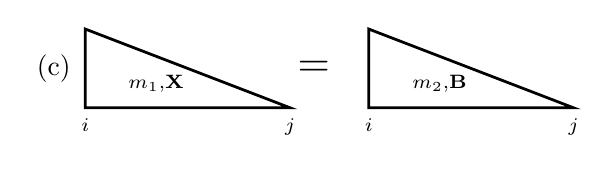
\begin{tikzpicture}
		\node [scale = 1](a) at (-0.6,0.5) {(c)};
		\draw [line width = 1pt] (2.4,0) node [below] {\scriptsize $j$} -- (-0.2,0) node [below] {\scriptsize $i$} -- (-0.2,1) -- cycle;
		\node [](pa_type1) at (0.7, 0.3) {\scriptsize $m_1$,$\mathbf{X}$};
		\node [scale = 1.5](equals) at (2.7, 0.5) {=};
		\draw [line width = 1pt] (6.0,0) node [below] {\scriptsize $j$} -- (3.4,0) node [below] {\scriptsize $i$} -- (3.4,1)-- cycle;
		\node [](type) at (4.3, 0.3) {\scriptsize $m_2$,$\mathbf{B}$};
		\end{tikzpicture}
	\end{subfigure}
	\begin{subfigure}{0.6\linewidth}
		
		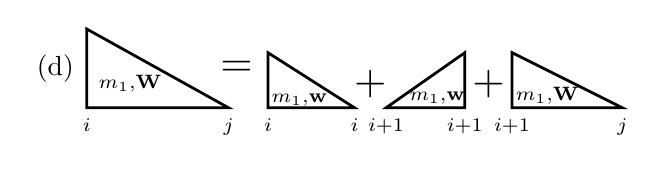
\begin{tikzpicture}
		\node [scale = 1](a) at (-0.6,0.5) {(d)};
		\draw [line width = 1pt] (1.6,0) node [below] {\scriptsize $j$} -- (-0.2,0) node [below] {\scriptsize $i$} -- (-0.2,1) -- cycle;
		\node [](type) at (0.35, 0.3) {\scriptsize $m_1$$,$$\mathbf{W}$};
		\node [scale = 1.5](equals) at (1.7,0.5) {=};
		\draw [line width = 1pt] (3.2,0) node [below] {\scriptsize $i$} -- (2.1,0.0) node [below] {\scriptsize $i$}-- (2.1,0.7) -- cycle;
		\node [](pa_type1) at (2.5, 0.1) {\scriptsize $m_1$$,$$\mathbf{w}$};
		\node [scale = 1.5](equals) at (3.4,0.3) {+};
		\draw [line width = 1pt] (4.6,0) node [below] {\scriptsize $i$$+$$1$} -- (3.6,0) node [below] {\scriptsize $i$$+$$1$} -- (4.6,0.7) -- cycle;
		\node [](pa_type2) at (4.25, 0.12) {\scriptsize $m_1$$,$$\mathbf{w}$};
		\node [scale = 1.5](equals) at (4.9,0.3) {+};
		\draw [line width = 1pt] (6.6,0) node [below] {\scriptsize $j$} -- (5.2,0.0) node [below] {\scriptsize $i$$+$$1$}-- (5.2,0.7) -- cycle;
		\node [](pa_type2) at (5.65, 0.15) {\scriptsize $m_1$$,$$\mathbf{W}$};
		\end{tikzpicture}
	\end{subfigure}
	%	\vspace{-2mm}
	\caption{The dynamic-programing structures and derivation of our model. The other direction is symmetric. See supplementary material for the complete structures.}
	%	\vspace{-3.8mm}
	\label{fig:modelderivation}
\end{figure}



As we can see from the derivation in Figure \ref{fig:modelderivation}, each type of span can be constructed from smaller spans in a bottom-up manner.  
Figure \ref{fig:modelderivation}a shows that a {complete span} is constructed from a {complete arc span} following the dependency patterns in Table \ref{tab:patterns}. 
Figure \ref{fig:modelderivation}b shows a {complete arc span} can be simply constructed from two smaller complete spans based on the dependency pattern.  
In Figure \ref{fig:modelderivation}c and \ref{fig:modelderivation}d, we further show how such two complete spans with pattern $\mathbf{X}$ (or $\mathbf{Y}$) and $\mathbf{W}$ can be constructed.
Figure \ref{fig:modelderivation}c illustrates how to model a transition from one semantic unit to another where the parent is $m_1$ and the child is $m_2$ in the semantic tree. 
If $m_2$ has arity 1, then the pattern is $\mathbf{B}$ following the dependency patterns in Table \ref{tab:patterns}. 
For spans with a single word, we use the lowercase $\mathbf{w}$ as the pattern to indicate this fact, as shown in Figure \ref{fig:modelderivation}d. 
They are the atomic spans used for building larger spans. 
As the {complete span} in Figure \ref{fig:modelderivation}d is associated with pattern $\mathbf{W}$, which means the words within this span are under the semantic unit $m_1$, we can incrementally construct this span with atomic spans.
We illustrate the construction of a complete dependency-based hybrid tree in the supplementary material. 


Our final goal during training for a sentence $\boldsymbol{n}=\{w_0, w_1,\cdots, w_N\}$ is to construct all the possible {\em complete spans} that cover the interval $[0, N]$, which can be represented as $C_{0,N,\cdot, \cdot}$. 
Similar to the chart-based dependency parsing algorithms~\cite{eisner1996three,eisner2000bilexical,koo2010efficient}, we can obtain the {\em inside} and {\em outside} scores using our dynamic-programming derivation in Figure \ref{fig:modelderivation} during the inference process,
which can then be used to calculate the objective and feature expectations. 
Since the spans are defined by at most three free indices, the dependency pattern and the semantic unit, our dynamic-programming algorithm requires $\mathcal{O}(N^3M)$ time\footnote{We omit a small constant factor associated with patterns.} where $M$ is the number of semantic units. 
The resulting complexity is the same as the {relaxed hybrid tree} model~\cite{lu2014semantic}. 

%the number of pattern as it is small as shown in Table \ref{tab:patterns}.

%We use $\alpha ( C_{i,j,p,m} )$ denotes the {\em inside} scores (in exponential space) of all the possible dependency-based hybrid trees that are rooted at $m$, with word association pattern $p$ and covering span $(w_i, \cdots, w_j)$. 
%
%We use Figure \ref{fig:dhtexample}a and \ref{fig:dhtexample}b to illustrate how these scores are computed using the dynamic programming structures. 
%The {\em inside} score derivations are similar to the one in {\em relaxed hybrid tree}~\cite{lu2014semantic} and dynamic-programing-based dependency parsing~\cite{koo2010efficient,shi2017fast}. 
%\begin{equation}
%\begin{split}
%\alpha (C^r_{i,j,p,m})  & = \sum_{p^\prime \in children(p)} \sum_{k=i+1}^{j} \alpha(A^r_{i,k,j,p^\prime,m}) \\
%\alpha(A^r_{i,k,j,p,m}) & = \alpha (C^l_{i+1, k, pc_1, m}) \otimes  \alpha (C^r_{k, j, pc_1, m})  \nonumber 
%\end{split}
%\end{equation}
%where the $\otimes$ operation 
%
%Finally, the inside score for a specific span $n= (w_i, \cdots, w_j)$ rooted at $m$ can be calculated by:
%\begin{equation}
%\alpha \big( C^r_{i, j,\cdot,m}\big) = \sum_p \alpha \big( C^r_{i, j,p,m}\big)
%\end{equation}
%
%
%
%It is clear to see that the above dynamic-programming algorithm have a complexity of $\mathcal{O}(n^3T)$ where $T$ is the number of semantic units and the complexity is same as the \textit{hybrid tree} model~\cite{lu2014semantic}. 
%
%For a sentence $\vec{n}$ with 

During decoding, we can find the optimal (tree-structured) meaning representation $\boldsymbol{m}^*$ for a given  input sentence $\boldsymbol{n}$ by the Viterbi algorithm. 
This step can also be done efficiently with our dynamic-programming approach, where we switch from marginal inference to MAP inference:
\begin{equation}
\boldsymbol{m}^*, \boldsymbol{t}^* = \argmax_{\boldsymbol{m}, \boldsymbol{t}\in\mathcal{T} (\boldsymbol{n}, \boldsymbol{m})} e ^{\vec{w} \cdot \vec{f} (\boldsymbol{n}, \boldsymbol{m}, \boldsymbol{t})}
\end{equation}
%\begin{center}
%	\begin{tabular}{c}
%		$
%		 \boldsymbol{m}^*, \boldsymbol{t}^* = \argmax_{\boldsymbol{m}, \boldsymbol{t}\in\mathcal{T} (\boldsymbol{n}, \boldsymbol{m})} e ^{\vec{w} \cdot \vec{f} (\boldsymbol{n}, \boldsymbol{m}, \boldsymbol{t})}
%		$
%	\end{tabular}
%\end{center}
%\begin{equation}
%\begin{split}
%\boldsymbol{m}^*, \boldsymbol{t}^* 
%%& = \argmax_{\boldsymbol{m}, \boldsymbol{t}\in\mathcal{T} (\boldsymbol{n}, \boldsymbol{m})}  P_\vec{w}(\boldsymbol{m}, \boldsymbol{t} | \boldsymbol{n}) \\
%& = \argmax_{\boldsymbol{m}, \boldsymbol{t}\in\mathcal{T} (\boldsymbol{n}, \boldsymbol{m})} e ^{\vec{w} \cdot \vec{f} (\boldsymbol{n}, \boldsymbol{m}, \boldsymbol{t})}
%\end{split}
%\end{equation}
%\begin{equation}
%\begin{split}
%\vec{m}^* & = \argmax_\vec{m} P_\vec{w}(\vec{m} | \vec{n}) \\
%& = \argmax_\vec{m} \sum_{\vec{t} \in \mathcal{T} (\vec{n}, \vec{m})} 
%P_\vec{w}(\vec{m}, \vec{t} | \vec{n}) \\
%& = \argmax_\vec{m} \sum_{\vec{t} \in \mathcal{T} (\vec{n}, \vec{m})}  
%e ^{\vec{w} \cdot \vec{f} (\vec{n}, \vec{m}, \vec{t})}
%\end{split}
%\end{equation}
%In order to use a dynamic-programming procedure similar to the training process, we replace the $\sum$ operation with $\max$. 
%We can jointly find the optimal meaning representation $\vec{m}^*$ together with the optimal dependency tree $\vec{t}$ by the following:
%\begin{equation}
%\begin{split}
%\vec{m}^*, \vec{t}^* 
%& = \argmax_{\vec{m}, \vec{t}\in\mathcal{T} (\vec{n}, \vec{m})}  e ^{\vec{w} \cdot \vec{f} (\vec{n}, \vec{m}, \vec{t})} \\
%& = \argmax_{\vec{m}, \vec{t}\in\mathcal{T} (\vec{n}, \vec{m})} \vec{w} \cdot \vec{f} (\vec{n}, \vec{m}, \vec{t})
%\end{split}
%\end{equation}
A similar decoding procedure has been used in previous work~\cite{lu2014semantic,durrett2015neural} with CKY-based parsing algorithm.
%The underlying procedure was also used in previous work~\cite{lu2014semantic,susanto2017semantic}. 
%We can then use Viterbi algorithm find the optimal meaning representation $\vec{m}^*$ as well as the optimal dependency tree $\vec{t}^*$ that contains the $\vec{m}^*$. 

%{\color{red}
%}







\subsection{Features}
\label{sec:features}
As shown in Equation \ref{equ:joint}, the features are defined on the tuple $(\boldsymbol{n}, \boldsymbol{m}, \boldsymbol{t})$. 
With the dynamic-programming procedure, we can define the features over the structures in Figure \ref{fig:dhtexample}. 
Our feature design is inspired by the {hybrid tree} model~\cite{lu2015constrained} and graph-based dependency parsing~\cite{mcdonald2005online}. 
Table \ref{tab:features} shows the feature templates for the example in Figure \ref{fig:dhtexample}. 
Specifically, we define simple unigram features (concatenation of a semantic unit and a word that directly appears under the unit), pattern features (concatenation of the semantic unit and the child pattern) and transition features (concatenation of the parent and child semantic units). 
They form our basic feature set. 


\begin{table}[t!]
	\centering
%	\scalebox{1.0}{
		\begin{tabular}{lc}
			\toprule
			Feature Type & Examples \\
			\midrule
			\midrule
			Word &  ``$m_4$ \& {\em run}'', ~~``$m_4$ \& {\em through}'' \\
			Pattern & ``$m_2$ \& $\mathbf{XY}$'', ~~``$m_4$ \& $\mathbf{WX}$'' \\
			Transition & ``$m_2$ \& $m_3$'', ~~``$m_2$ \& $m_4$'' \\
			\midrule
			\midrule 
			Head word & ``$m_2$ \& {\em What}'', ~~``$m_4$ \& {\em not}'' \\
			Modifier word & ``$m_2$ \& {\em not}'', ~~``$m_4$ \& {\em through}'' \\
			Bag of words & ``$m_4$ \& {\em not}'', ~~``$m_4$ \& {\em run}'', ~~``$m_4$ \& {\em through}'' \\
			\bottomrule 
		\end{tabular}
%	}
	%	\vspace{-2mm}
	\caption{Features for the example in Figure \ref{fig:dhtexample}. 
		%	Bottom shows the dependency-related features.
	}
	%	\vspace{-3mm}
	\label{tab:features}
\end{table}

Additionally, with the structured properties of dependencies, we can define dependency-related features~\cite{mcdonald2005online}. 
%We use the parent and child words head (parent) and modifier (child) words of the dependency as features. 
We use the parent (head) and child (modifier) words of the dependency as features.
We also use the bag-of-words covered under a dependency as features. 
The dependency features are useful in helping improve the performance as we can see in the experiments section. 
%We present  examples of features in the supplementary material.



\subsection{Neural Component}

Following the approach used in \citet{susanto2017semantic}, we could further incorporate  neural networks into our latent-variable graphical model. 
The integration is analogous to the approaches described in the neural CRF models~\cite{artieres2010neural,durrett2015neural,gormley2015graphical,lample2016neural},
where we use neural networks to learn distributed feature representations within our graphical model.

%\begin{figure}[t!]
%	\centering
%	\begin{tikzpicture}[node distance=4mm and 4mm, >=Stealth, 	place/.style={draw=none, inner sep=2pt,line width=0.8pt},
%	invis/.style={draw=none, circle,line width=0pt, inner sep=0pt, fill=none, text=fontgray}]
%	\node [place](wleft) [] {$w_{p}$};
%	
%	
%	\node [draw, line width=0.8pt, rectangle, minimum width=0.4pt, minimum height=20pt, rounded corners=0.2pt] (wleftembed) [right=of wleft] {};
%	\node [draw, line width=0.8pt, rectangle, minimum width=0.4pt, minimum height=20pt, rounded corners=0.2pt] (wrightembed) [below=of wleftembed] {};
%%	\node [place](wmiddle) [left=of wmiddleembed] {$w_{t}$};
%	\node [place](wright) [left=of wrightembed] {$w_{c}$};
%	
%	\draw [line width=0.8pt, ->] (wleft) to [] node [] {} (wleftembed);
%%	\draw [line width=1pt, ->] (wmiddle) to [] node [] {} (wmiddleembed);
%	\draw [line width=0.8pt, ->] (wright) to [] node [] {} (wrightembed);
%	
%	%hidden layer
%	\node [draw, line width=0.8pt, rectangle, text width=11mm, minimum height=50pt, rounded corners=1pt,xshift=5mm, yshift=-4mm] (hidden) [right=of wleftembed] {\small Bilinear\\~~~$\mathbf{U}$};
%	\node [place, text width=23pt, font=\small, align=center, yshift =3mm](hiddenword) [below=of hidden] {};
%	
%	\draw [line width=0.8pt, ->] (wleftembed) to [] node [above, font=\small] {$\vec{e}_{p}$} (hidden);
%%	\draw [line width=1pt, ->] (wmiddleembed) to [] node [above, font=\small, yshift=-1mm, xshift=-1mm] {$\vec{e}_{t}$} (hidden);
%	\draw [line width=0.8pt, ->] (wrightembed) to [] node [below, font=\small, xshift=1mm] {$\vec{e}_{c}$} (hidden);
%	
%	\node [draw=none, line width=0.8pt, minimum width=0.4pt, minimum height=50pt, rounded corners=1pt,xshift=5mm] (output) [right=of hidden] {};
%%	\node [place, text width=23pt, font=\small, align=center, yshift =3mm](outputword) [below=of output] {output layer};
%	\draw [line width=0.8pt, ->] (hidden) to [] node [above] {} (output);
%	
%	\end{tikzpicture}
%	\caption{Our bilinear neural architecture.}
%	\label{fig:neural}
%\end{figure}
%As the semantic units are defined on the dependencies, w
We employ a neural architecture to calculate the score associated with each dependency arc $(w_p, w_c, m)$ (here $w_p$ and $w_c$ are the parent and child words in the dependency and $m$ is the semantic unit over the arc), where the input to the neural network consists of  words (i.e., $(w_p, w_c)$) associated with this dependency and the neural network will calculate a score for each possible semantic unit, including $m$.
% the score of the semantic unit $m$. 
The two words are first mapped to word embeddings  $\vec{e}_p$ and $\vec{e}_c$ (both of dimension $d$). 
Next, we use a bilinear layer\footnote{Empirically, we also tried multilayer perceptron but the bilinear model gives us better results.}~\cite{socher2013recursive,chen2016thorough} to capture the interaction between the parent and the child in a dependency:
\begin{equation*}
r_i = \vec{e}_p^{\mathbf{T}} \mathbf{U}_i \vec{e}_c
\end{equation*}
%\begin{center}
%	\begin{tabular}{c}
%		$
%		r_i = \vec{e}_p^{\mathbf{T}} \mathbf{U}_i \vec{e}_c
%		$
%	\end{tabular}
%\end{center}
where $r_i$ represents the score for the $i$-th semantic unit and $\mathbf{U}_i \in \mathbb{R}^{d\times d}$.
The scores are then incorporated into the probability expression in Equation \ref{equ:joint} during learning and decoding.
As a comparison, we also implemented a  variant where our model directly takes in the average embedding of $\mathbf{e}_p$ and $\mathbf{e}_c$ as additional features, without using our neural component. 

%We implemented two neural architectures: multilayer perceptron (MLP) and bilinear networks. 
%The MLP architecture is also used in the {\it neural hybrid tree} model~\cite{susanto2017semantic}. 
%However, the window size in their MLP can differ in terms of the language, which may not be robust. 
%Our MLP and bilinear architectures do not require the window size. 






\section{Experiments}

\paragraph{Data and evaluation methodology} 

We conduct experiments on the publicly available variable-free version of the GeoQuery dataset, which has been widely used for semantic parsing~\cite{wong2006learning,lu2008generative,jones2012semantic}. 
The dataset consists of 880 pairs of natural language sentences and the corresponding tree-structured semantic representations. 
This dataset is annotated with eight languages. 
%This dataset is annotated with eight languages~\cite{jones2012semantic,lu2011probabilistic,susanto2017semantic}.  
The original annotation of this dataset is English~\cite{zelle1996learning} and \citet{jones2012semantic} annotated the dataset with three more languages: German, Greek and Thai. 
\citet{lu2011probabilistic} released the Chinese annotation and \citet{susanto2017semantic} annotated the corpus with three additional languages: Indonesian, Swedish and Farsi. 
In order to compare with previous work~\cite{jones2012semantic,lu2015constrained}, we follow the standard splits with 600 instances for training and 280 instances for testing. 
To evaluate the performance, we follow the standard evaluation procedure used in various previous works \cite{wong2006learning,lu2008generative,jones2012semantic,lu2015constrained} to construct the Prolog query from the tree-structured semantic representation using a standard and publicly available script. 
The queries are then used to retrieve the answers from the GeoQuery database, and we report  accuracy and $F_1$ scores.
% based on the retrieved answers. 

\paragraph{Hyperparameters} 
We set the maximum depth $c$ of the semantic tree to 20, following \citet{lu2015constrained}. 
The $L_2$ regularization coefficient is tuned from 0.01 to 0.05 using 5-fold cross-validation on the training set.
The Polyglot~\cite{polyglot:2013:ACL-CoNLL} multilingual word embeddings\footnote{The embeddings are fixed to avoid overfitting.} (with 64 dimensions) are used for all languages.  
We use L-BFGS~\cite{liu1989limited} to optimize the \textsc{DepHT} model until convergence 
and stochastic gradient descent (SGD) with a learning rate of 0.05 to optimize the neural \textsc{DepHT} model.
% with 20 epochs. 
We implemented our neural component with the Torch7 library~\cite{collobert2011torch7}. 
Our complete implementation is based on the StatNLP\footnote{https://gitlab.com/sutd\_nlp/statnlp-core} structured prediction framework~\cite{lu2017unified}. 


\subsection{Baseline Systems}

We run the released systems of several state-of-the-art semantic parsers, namely the \textsc{Wasp} parser~\cite{wong2006learning}, \textsc{HybridTree} model~\cite{lu2008generative}, \textsc{UBL} system~\cite{kwiatkowski2010inducing},  \textit{relaxed hybrid tree} (\textsc{RHT})~\cite{lu2015constrained}\footnote{\cite{lu2015constrained} is an extension of the original \textit{relaxed hybrid tree}~\cite{lu2014semantic}, which reports improved results.}, the sequence-to-tree (\textsc{Seq2Tree}) model~\cite{dong2016language}, the \textit{neural hybrid tree} (\textsc{Neural HT}) model~\cite{susanto2017semantic}, and the multilingual semantic parser~\cite{susanto2017neural} with single language (\textsc{MSP-Single}) as input. 
The results for \textsc{TreeTrans}~\cite{jones2012semantic} are taken from their paper.


\subsection{Results and Discussion}



Table \ref{tab:nonneuralresults} (top) shows the results of our {dependency-based hybrid tree} model compared with non-neural models which achieve state-of-the-art performance on the GeoQuery dataset. 
Our model \textsc{DepHT} achieves competitive performance and outperforms the previous best system \textsc{RHT} on 6 languages.

\begin{table*}[h!]
	\centering
	\resizebox{1\linewidth}{!}{
		\begin{tabular}{clcccccccccccccccc}
			\toprule
			\multirow{2}{*}{Type}&\multirow{2}{*}{System/Model} & \multicolumn{2}{c}{English (en)}& \multicolumn{2}{c}{Thai (th)}& \multicolumn{2}{c}{German (de)}& \multicolumn{2}{c}{Greek (el)}& \\
			&& \textit{Acc.} & \textit{F.}& \textit{Acc.} & \textit{F.}& \textit{Acc.} & \textit{F.}& \textit{Acc.} & \textit{F.} \\
			\midrule
			\midrule 
			\multirow{5}{*}{Non-Neural}&\textsc{Wasp}  & 71.1 & 77.7 & 71.4 & 75.0 & 65.7 & 74.9 & 70.7 & 78.6  \\
			&\textsc{HybridTree}  & 76.8 & 81.0 & 73.6 & 76.7 & 62.1 & 68.5 & 69.3 & 74.6 6 \\
			&\textsc{UBL}  & 82.1 & 82.1 & 66.4 &66.4 & 75.0 & 75.0 & 73.6 &73.7 \\
			&\textsc{TreeTrans}  & 79.3 & 79.3 & 78.2 &78.2 & 74.6 &74.6 & 75.4 &75.4 \\
			&\textsc{RHT}  & 86.8 & 86.8 & 80.7 & 80.7 &75.7 & 75.7 & 79.3 & 79.3\\\midrule 
			%			\textsc{DepHT} & {\bf 86.8} & {\bf 86.8} & {\bf 81.8} & {\bf 81.8} & {\bf 76.1} & {\bf 76.1} & {\bf 80.4} & {\bf 80.4} & \textbf{81.4} & \textbf{81.4}& {\bf 86.8} & {\bf 86.8} & {\bf 85.4} & {\bf 85.4} & {\bf 73.9} & {\bf 73.9}    \\
			\midrule 
			\multirow{5}{*}{Neural}&\textsc{Seq2Tree}$\dagger$  & 84.5 & - & 71.9 & - & 70.3 & - & 73.1 & -  \\
			&\textsc{MSP-Single}$\dagger$ & 83.5 & - & 72.1 & - & 69.3 & - &74.2 & -  \\
			&\textsc{Neural HT} ($J$=0)&  87.9&87.9  &82.1 &82.1 &75.7&75.7 &81.1 &81.1\\
			&\textsc{Neural HT} ($J$=1)&88.6  &88.6 &84.6 &84.6  &76.8 &76.8 &79.6 &79.6 \\
			&\textsc{Neural HT} ($J$=2)& \textbf{90.0} &\textbf{90.0}  &  82.1&82.1  & 73.9&73.9 &80.7 &80.7\\ \midrule\midrule
			Non-Neural&(This work) \textsc{DepHT}  & 86.8 & 86.8 & 81.8 & 81.8 & 76.1 & 76.1 & 80.4 & 80.4    \\
			Non-Neural&(This work) \textsc{DepHT} + embedding & 87.5 & 87.5 &83.9 & 83.9 & 75.0 & 75.0 & 81.1 & 81.1   \\
			%			\textsc{DepHT} + MLP &  &  & &  & &&  & & & &  &  & &  & &     \\ 
			%			\textsc{DepHT} + MLP& 88.2 & 88.2 &  & & &&  & & & &  &  & &  & & \\
			Neural&(This work) \textsc{DepHT} + NN  & 89.3 & 89.3 & \textbf{86.7} & \textbf{86.7}& {\bf 78.2} & {\bf 78.2} &  {\bf 82.9}& {\bf 82.9} \\
			\bottomrule
		\end{tabular}
	}
	%	\vspace{-2mm}
	\caption{Performance comparison with state-of-the-art models on GeoQuery dataset. ($\dagger$ represents the system is using lambda-calculus expressions as meaning representations.)}
	\label{tab:nonneuralresults}
	%	\vspace*{-1mm}
\end{table*}

\begin{table*}[h!]
	\centering
	\resizebox{1\linewidth}{!}{
		\begin{tabular}{clcccccccc}
			\toprule
			\multirow{2}{*}{Type}&\multirow{2}{*}{System/Model} & \multicolumn{2}{c}{Chinese (zh)}& \multicolumn{2}{c}{Indonesian (id)}& \multicolumn{2}{c}{Swedish (sv)}& \multicolumn{2}{c}{Farsi (fa)} \\
			&& \textit{Acc.} & \textit{F.}& \textit{Acc.} & \textit{F.}& \textit{Acc.} & \textit{F.}& \textit{Acc.} & \textit{F.} \\
			\midrule
			\midrule 
			\multirow{5}{*}{Non-Neural}&\textsc{Wasp}   & 48.2 & 51.6 & 74.6 & 79.8 & 63.9 & 71.5 & 46.8 & 54.1 \\
			&\textsc{HybridTree}  & 56.1 & 58.4 & 66.4 & 72.8 & 61.4 & 70.5 & 51.8 & 58.6 \\
			&\textsc{UBL}  & 63.8 & 63.8 & 73.8 & 73.8 & 78.1 & 78.1 &64.4 & 64.4\\
			&\textsc{TreeTrans}   & - & - &- & -&- & -&- & -\\
			&\textsc{RHT}  & 76.1 & 76.1 & 75.0 & 75.0 &  79.3 & 79.3 &  73.9 & 73.9\\\hline 
			%			\textsc{DepHT} & {\bf 86.8} & {\bf 86.8} & {\bf 81.8} & {\bf 81.8} & {\bf 76.1} & {\bf 76.1} & {\bf 80.4} & {\bf 80.4} & \textbf{81.4} & \textbf{81.4}& {\bf 86.8} & {\bf 86.8} & {\bf 85.4} & {\bf 85.4} & {\bf 73.9} & {\bf 73.9}    \\
			\midrule 
			\multirow{5}{*}{Neural}&\textsc{Seq2Tree}$\dagger$  & 73.3 & - & 80.7 & - & 80.8 & - & 70.5 & - \\
			&\textsc{MSP-Single}$\dagger$  & 74.9 & - & 79.8 & - & 77.5 & - & 72.2 & - \\
			&\textsc{Neural HT} ($J$=0)76.8&76.8&76.1&76.1&81.1&81.1&75.0&75.0 \\
			&\textsc{Neural HT} ($J$=1)&75.4&75.4&78.6&78.6&82.9&82.9&76.1 &76.1 \\
			&\textsc{Neural HT} ($J$=2)&81.1&81.1&{81.8}&{81.8}&83.9&83.9&74.6&74.6\\ \hline\hline
			Non-Neural&(This work) \textsc{DepHT}   & 81.4 & 81.4& 86.8 & 86.8 & 85.4 & 85.4 & 73.9& 73.9    \\
			Non-Neural&(This work) \textsc{DepHT} + embedding  & 81.4 & 81.4& 87.5 & 87.5 & 87.1 & 87.1 & 73.6 & 73.6    \\
			%			\textsc{DepHT} + MLP &  &  & &  & &&  & & & &  &  & &  & &     \\ 
			%			\textsc{DepHT} + MLP& 88.2 & 88.2 &  & & &&  & & & &  &  & &  & & \\
			Neural&(This work) \textsc{DepHT} + NN  & {\bf 82.9} & {\bf 82.9} & {\bf 88.7} & {\bf 88.7} & {\bf 87.3} & {\bf 87.3} & {\bf 77.9}& {\bf 77.9} \\
			\bottomrule
		\end{tabular}
	}
	%	\vspace{-2mm}
	\caption{Performance comparison with state-of-the-art models on GeoQuery dataset. ($\dagger$ represents the system is using lambda-calculus expressions as meaning representations.)}
	\label{tab:nonneuralresults2}
	%	\vspace*{-1mm}
\end{table*}



Improvements on the Indonesian dataset are particularly striking (+11.8 absolute points in $F_1$).
We further investigated the outputs from both systems on Indonesian by doing error analysis.
% for those wrong predictions by \textsc{RHT} but correctly predicted by our \textsc{DepHT}.  
We found 40 instances that are incorrectly predicted by \textsc{RHT} are correctly predicted by \textsc{DepHT}. 
%We summarize three types of errors made by the \textsc{RHT} model in Table \ref{tab:errors}. 
We found that 77.5\% of the errors are due to incorrect alignment between words and semantic units as shown in Table \ref{tab:errors}.

\begin{table}[h!]
	\centering
	
	\begin{tabular}{lc}
		\toprule 
		Error Cause & \% \\\midrule
		Missing semantic unit & 12.5\\
		Incorrect semantic unit & 10.0\\
		Incorrect alignment & 77.5\\
		\bottomrule 
	\end{tabular}
	
	%	\vspace{-2mm}
	\caption{Different types of errors in the prediction of {\em relaxed hybrid tree} model. }
	%	\vspace{-2mm}
	\label{tab:errors}
\end{table}

% incorrect alignment. 
Figure \ref{fig:indoerror} shows an example of such errors where the relaxed hybrid tree fails to capture the correct alignment.


\begin{figure}[t!]
	\centering
	\scalebox{1}{
		\begin{tikzpicture}[node distance=2.0mm and 2.5mm, >=Stealth, 
		semantic/.style={draw=none, minimum height=5mm, rectangle},
		word/.style={draw=none, minimum height=5mm, rectangle},
		olabel/.style={draw=none, circle, minimum height=9mm, minimum width=9mm,line width=1pt, inner sep=2pt, fill=lowblue, text=fontgray, label={center:\textsc{o}}},
		bperlabel/.style={draw=none, circle, minimum height=9mm, minimum width=9mm,line width=1pt, inner sep=2pt, fill=lowblue, text=black, label={center:\textsc{per}}},
		borglabel/.style={draw=none, circle, minimum height=9mm, minimum width=9mm,line width=1pt, inner sep=2pt, fill=lowblue, text=black, label={center:\textsc{org}}},
		bgpelabel/.style={draw=none, circle, minimum height=9mm, minimum width=9mm,line width=1pt, inner sep=2pt, fill=lowblue, text=black, label={center:\textsc{Misc}}},
		nnlabel/.style={draw=none, circle, minimum height=9mm, minimum width=9mm,line width=1pt, inner sep=2pt, fill=mypumpkin, text=black, label={center:\textsc{Gpe}}},
		invis/.style={draw=none, circle, minimum height=9mm, minimum width=9mm,line width=1pt, inner sep=2pt, fill=none, text=fontgray},
		chainLine/.style={line width=0.8pt,->, color=fontgray}	%		,background rectangle/.style={fill=olive!45}, show background rectangle
		]
		\node[semantic](sent) [] {Sentence: {\em San ~~~~~ Antonio ~~~~ berada ~~~~ di ~~~~ negara ~~~~~ bagian ~~~~ apa ~~~~~ ?}}; 
		\node[word](ew0) [below left= of sent,xshift=28.2mm,yshift=4mm] {({\em San})}; 
		\node[word](ew1) [right = of ew0, xshift=-1mm] {({\em Antonio})};
		\node[word](ew2) [right = of ew1, xshift=-2mm] {({\em located})};
		\node[word](ew3) [right = of ew2, xshift=-2.5mm] {({\em in})};
		\node[word](ew4) [right = of ew3, xshift=-1.9mm] {({\em ~~~~~~~~~~~state~~~~~~~~~~~})};
		%		\node[word](ew5) [right = of ew4, xshift=-2mm] {(})}; 
		\node[word](ew6) [right = of ew4, xshift=-2.6mm] {({\em what})}; 
		\node[word](ew7) [right = of ew6, xshift=-2mm] {({\em ?})}; 
		
		\node[word](correctsem) [below = of sent, yshift=-2mm] {Gold Meaning Representation: $answer(loc(cityid('san\;antonio')))$};
		
		\node[word](htname) [below = of correctsem, xshift=-20mm, yshift=-1mm] {{\em Relaxed Hybrid Tree}};
		
		\node[word](hm1) [below = of htname, xshift=0mm] {$m_1$};
		\node[word](hw1) [below left = of hm1, xshift=0mm, yshift=-3mm] {{\em San Antonio breada di}};
		\node[word](hw5) [below right = of hm1, xshift=9mm, yshift=-3mm] {{\em ?}};
		\node[word](hm2) [below= of hm1, xshift=0mm, yshift=-3mm] {$m_4$};
		
		%		\node[word](hm3) [below left= of hm2, xshift=-8mm, yshift=-3mm] {$m_3$};
		%		\node[word](hm4) [below = of hm2, xshift=0mm, yshift=-3mm] {$m_4$};
		\node[word](hw34) [below= of hm2, xshift=0mm, yshift=-3mm] {{\em negara bagian apa}};
		
		%		\node[word](hw2) [below= of hm3, xshift=0mm, yshift=-3mm] {{\em rivers}};
		
		%		\node[word](hm5) [below right= of hm4, xshift=5mm, yshift=-3mm] {$m_5$};
		%		\node[word](hw4) [below left= of hm5, xshift=0mm, yshift=0mm] {{\em di}};
		%		\node[word](hw56) [below left= of hm4, xshift=5mm, yshift=-3mm] {{\em titik tertinggi}};
		%		\node[word](hm6) [below= of hm5, xshift=0mm, yshift=-3mm] {$m_6$};
		%		\node[word](hm7) [below= of hm6, xshift=0mm, yshift=-3mm] {$m_7$};
		%		\node[word](hw5) [below right= of hm6, xshift=0mm, yshift=0mm] {{\em ?}};
		%		\node[word](hwiowa) [below= of hm7, xshift=0mm, yshift=-3mm] {{\em iowa}};
		
		\draw [chainLine] (hm1) to [] node[] {} (hw1);
		\draw [chainLine] (hm1) to [] node[] {} (hm2);
		\draw [chainLine] (hm1) to [] node[] {} (hw5);
		
		\draw [chainLine] (hm2) to [] node[] {} (hw34);
		%		\draw [chainLine] (hm2) to [] node[] {} (hw34);
		%		\draw [chainLine] (hm2) to [] node[] {} (hm4);
		%		
		%		\draw [chainLine] (hm5) to [] node[] {} (hw4);
		%		\draw [chainLine] (hm4) to [] node[] {} (hw56);
		%		\draw [chainLine] (hm4) to [] node[] {} (hm5);
		%		
		%		\draw [chainLine] (hm5) to [] node[] {} (hm6);
		%		\draw [chainLine] (hm6) to [] node[] {} (hm7);
		%		\draw [chainLine] (hm6) to [] node[] {} (hw5);
		%		\draw [chainLine] (hm7) to [] node[] {} (hwiowa);
		
		
		
		%		\node[word](root) [below = of dhtname, xshift=0mm] {\textit{root}};
		%		\node[word](what) [below left = of root, yshift=-3mm, xshift=-3mm] {\textit{What}};
		%		%		\node[invis](rootop) [above = of w0, yshift=8mm] {};
		%		\node[word](not) [below right = of what, xshift=15mm, yshift=3mm] {\textit{not}};
		%		\node[word](rivers) [below left = of not, yshift=-4mm] {\textit{rivers}};
		%		\node[word](through) [below right = of not, yshift=-4mm] {\textit{through}};
		%		\node[word](tennessee) [below right = of through, yshift=-4mm, xshift=-2mm] {\textit{Tennessee}};
		
		\node[word](m1)[below= of htname, xshift=55mm, yshift=2mm] {$m_1$: Q{\small{UERY}} : $answer$ (S{\small{TATE}})};
		\node[word](m2)[below= of m1, yshift=4mm, xshift=-5.7mm] {$m_2$: S{\small{TATE}} : $loc$ (C{\small{ITY}})};
		\node[word](m3)[below= of m2, yshift=4mm, xshift=6.4mm] {$m_3$: C{\small{ITY}} : $cityid$ (C{\small{ITY}}N{\small{AME}})};
		\node[word](m4)[below= of m3, yshift=4mm, xshift=-6.4mm] {$m_4$: S{\small{TATE}} : $state$ ($all$)};
		%		\node[word](m5)[below= of m4, yshift=4mm, xshift=-2.2mm] {$m_5$: P{\small{LACE}} : $loc$ (S{\small{TATE}})};
		%		\node[word](m6)[below= of m5, yshift=4mm, xshift=8.0mm] {$m_6$: S{\small{TATE}} : $stateid$ (S{\small{TATE}}N{\small{AME}})};
		\node[word](m5)[below= of m4, yshift=4mm, xshift=8.3mm] {$m_5$: C{\small{ITY}}N{\small{AME}} : ($'san\;antonio'$)};
		
		%		\Tree [.\node(root){$m_1 \equiv $ Q{\small{UERY}} : $answer$ (R{\small{IVER}})}; [.{$m_2 \equiv $ R{\small{IVER}}: $exclude$ (R{\small{IVER}}, R{\small{IVER}})} {$m_3 \equiv$ R{\small{IVER}} : $state$ (all)} [.{$m_4 \equiv$ R{\small{IVER}} : $traverse$ (S{\small{TATE}})} [.{$m_5 \equiv $S{\small{TATE}} : $stateid$ (S{\small{TATE}}N{\small{AME}})} {$m_6 \equiv$  S{\small{TATE}}N{\small{AME}} : ($'texas'$)} ]] ]]
		
		%		\draw [chainLine] (root) to [] node[above, color=black,sloped] {\small  $m_1$} (what);
		%		\draw [chainLine] (what) to [] node[above, color=black,sloped] {\small  $m_2$} (not);
		%		\draw [chainLine] (not) to [] node[above, color=black,sloped] {\small  $m_3$} (rivers);
		%		\draw [chainLine] (not) to [] node[above, color=black,sloped] {\small  $m_4$} (through);
		%		\draw [chainLine] (through) to [] node[above, color=black,sloped] {\small  $m_5$} (tennessee);
		%		\draw [line width=0.8pt,->, color=fontgray]  (tennessee) to [out=90,in=-30, looseness=5.2] node[above, yshift=-1mm, color=black, sloped]{$m_6$} (tennessee);
		
		\node[word](wroot) [below = of sent, xshift = -55mm, yshift=-70mm] {{\em root}};
		\node[word](w0) [right = of wroot, xshift=2.5mm] {{\em San}};
		%		\node[invis](rootop) [above = of w0, yshift=8mm] {};
		\node[word](w1) [right = of w0, xshift=1mm] {{\em Antonio}};
		\node[word](w2) [right = of w1, xshift=1mm] {{\em berada}};
		\node[word](w3) [right = of w2, xshift=1mm] {{\em di}};
		\node[word](w4) [right = of w3, xshift=1mm, yshift=-1mm] {{\em negara}};
		\node[word](w5) [right = of w4, xshift=1mm] {{\em bagian}};
		\node[word](w6) [right = of w5, xshift=1mm] {{\em apa}};
		\node[word](w7) [right = of w6, xshift=1mm] {{\em ?}};
		\node[word](dhtname) [below = of sent, yshift=-48mm] {{\em Dependency-based Hybrid Tree}};
		\draw [line width=0.8pt,->, color=fontgray]  (wroot) to [out=48,in=132, looseness=0.9] node[above, yshift=-1mm, color=black]{$m_1$} (w3);
		\draw [line width=0.8pt,->, color=fontgray]  (w3) to [out=140,in=40, looseness=1] node[above, yshift=-1mm, xshift=-1mm, color=black]{$m_2$} (w2);
		\draw [line width=0.8pt,->, color=fontgray]  (w2) to [out=140,in=40, looseness=1] node[above, color=black, xshift= 0mm, yshift=-1mm]{$m_3$} (w1);
		%		\draw [line width=0.8pt,->, color=fontgray]  (w2) to [out=60,in=120, looseness=1] node[above, yshift=-1mm, color=black]{$m_5$} (w3);
		%		\draw [line width=0.8pt,->, color=fontgray]  (w3) to [out=60,in=120, looseness=1] node[above, yshift=-1mm, color=black]{$m_6$} (w4);
		\draw [line width=0.8pt,->, color=fontgray]  (w1) to [out=120,in=60, looseness=1] node[above, yshift=-1mm, color=black, xshift=0mm]{$m_5$} (w0);
		\end{tikzpicture} 
	}
	%	\vspace*{-3mm}
	\caption{Example results from \textsc{DepHT} and \textsc{RHT} on Indonesian.}
	%	\vspace*{-4mm}
	\label{fig:indoerror}
\end{figure}
%caused by the incorrect alignment in relaxed hybrid tree. 
We can see the question is asking ``{\em What state is San Antonio located in?}''. 
However, the natural language word order in Indonesian is different from English, where the phrase ``{\em berada di}'' that corresponds to $m_2$ (i.e., $loc$) appears between ``{\em San Antonio}'' (which corresponds to $m_5$ -- $'san\ antonio'$) and ``{\em what}'' (which corresponds to $m_1$ -- $answer$).
Such a structural non isomorphism issue between the sentence and the semantic tree  makes the relaxed hybrid tree parser unable to produce a joint representation with valid word-semantics alignment.
This issue makes the \textsc{RHT} model unable to predict the semantic unit $m_2$ (i.e., $loc$) as \textsc{RHT} has to align the words ``{\em San Antonio}'' which should be aligned to $m_5$ before aligning ``{\em berada di}''. 
However, $m_5$ has arity 0 and cannot have $m_2$ as its child. 
Thus, it would be impossible for the RHT model to predict such a meaning representation as output.
In contrast, we can see that our dependency-based hybrid tree representation appears to be more flexible in handling such cases. 
The dependency  between the two words ``{\em di}'' ({\em in}) and ``{\em berada}'' ({\em located}) is also well captured by the arc between them that is labeled with $m_2$.
%In our  {dependency-based hybrid tree} representation below, we can {\em directly} find the words ``{\em di}'' and ``{\em berada}'' where the dependency between them is represented by $m_2$. 
% due to the ordering of words in the sentences. 
The error analysis reveals the flexibility of our joint representation in different languages in terms of the word ordering, indicating that the novel dependency-based joint representation is more robust and suffers less from language-specific characteristics associated with the data.


\paragraph{Effectiveness of dependency}
To investigate the helpfulness of the features defined over latent dependencies, we conduct  ablation tests by removing the dependency-related features. 
Table \ref{tab:ablation} shows the performance of augmenting different dependency features in our \textsc{DepHT} model with basic features. 
Specifically, we investigate the performance of head word and modifier word features (\textsc{hm}) and also the bag-of-words features (\textsc{bow}) that can be extracted based on dependencies. 
It can be observed that dependency features  associated with the words are crucial for all languages, especially the \textsc{bow} features. 
\begin{table}[t!]
	\centering
%	\setlength{\tabcolsep}{3pt} % General space between cols (6pt standard)
	\renewcommand{\arraystretch}{1} % General space between rows (1 standard)
	\scalebox{1}{
		\begin{tabular}{lcccccccc}
			\toprule
			& en & th&de&el&zh&id&sv&fa\\\midrule
			\textsc{DepHT} basic & 75.0 &82.1 & 70.4&74.6&76.1&71.9&73.9&69.3\\ 
			\textsc{basic}+\textsc{hm} feats. & 80.7 & {\bf 83.9} & {\bf 75.7} &79.2&81.1&85.0&81.1&72.5\\
			\textsc{basic}+\textsc{bow} feats. & {\bf 86.1}&83.2&73.9&{\bf 79.3}&{\bf 81.4}& {\bf 86.1} &{\bf 85.4}&{\bf 73.2} \\
			\midrule
			\textsc{DepHT} & 86.8& 81.8& 76.1 & 80.4& 81.4& 86.8& 85.4& 73.9 \\
			\bottomrule
		\end{tabular}
	}
	\vspace*{-2mm}
	\caption{$F_1$ scores of our model with different dependency features.}
	\label{tab:ablation}
	\vspace*{-3mm}
\end{table}


\paragraph{Effectiveness of neural component}
The bottom part of Table \ref{tab:nonneuralresults} shows the performance comparison among models that involve neural networks.
Our \textsc{DepHT} model with embeddings as features can outperform neural baselines across several languages (i.e., Chinese, Indonesian and Swedish). 
From the table, we can see the neural component is effective, which consistently gives better results than \textsc{DepHT} and the approach that uses word embedding features only.
\citet{susanto2017semantic} presented the \textsc{Neural HT} model with different window size $J$ for their multilayer perceptron. Their performance will differ with different window sizes, which need to be tuned for each language. 
In our neural component, we do not require such a language-specific hyperparameter, yet our neural approach consistently achieves the highest performance on 7 out of 8 languages compared with all previous approaches.
% 
%With neural component, our model 
%As both the embedding and the neural component are defined on the dependency arc, the superior results of these model variants also reveal the effectiveness of our dependency-based hybrid tree representation in semantic parsing. 
As both the embeddings and the neural component are defined on the dependency arcs, the superior results also reveal the effectiveness of our dependency-based hybrid tree representation. 

%{\color{red}
%}


\section{Conclusions}

In this work, we present a novel {\em dependency-based hybrid tree} model for semantic parsing. 
The  model captures the underlying semantic information of a sentence as latent dependencies between the natural language words. 
We develop an efficient algorithm for exact inference  based on dynamic-programming.
Extensive experiments on benchmark dataset across 8 different languages demonstrate the effectiveness of our newly proposed representation for semantic parsing.

Future work includes exploring alternative approaches such as transition-based methods
%As we regard the semantics as dependencies, we would like to explore how to employ the efficient transition-based approach
~\cite{nivre2006maltparser,chen2014fast} for semantic parsing with latent dependencies, 
applying our dependency-based hybrid trees on other types of logical representations (e.g., lambda calculus expressions and SQL~\cite{P18-1033}) as well as multilingual semantic parsing~\cite{jie2014multilingual,susanto2017neural}.

\section{Dependency-based Hybrid Tree for SQL Parsing}

As SQL is getting popular recently, one natural question to ask is that \textit{Can we solve SQL parsing with Dependency-based Hybrid Trees?} 
Because the SQL itself is actually a sequential structure but not in a tree format, it could be difficult to solve it with dependency-based hybrid trees as well as designing certain grammar structures. 
However, sequential structure is a special tree structure where each node has only one child.
It is still possible to employ the dependency-based hybrid tree models for tackling the SQL problems. 
But we need to design different grammars and hybrid pattern under such a special meaning representation. 